% Options for packages loaded elsewhere
\PassOptionsToPackage{unicode}{hyperref}
\PassOptionsToPackage{hyphens}{url}
\documentclass[
  12pt,
]{article}
\usepackage{xcolor}
\usepackage[margin=1in]{geometry}
\usepackage{amsmath,amssymb}
\setcounter{secnumdepth}{-\maxdimen} % remove section numbering
\usepackage{iftex}
\ifPDFTeX
  \usepackage[T1]{fontenc}
  \usepackage[utf8]{inputenc}
  \usepackage{textcomp} % provide euro and other symbols
\else % if luatex or xetex
  \usepackage{unicode-math} % this also loads fontspec
  \defaultfontfeatures{Scale=MatchLowercase}
  \defaultfontfeatures[\rmfamily]{Ligatures=TeX,Scale=1}
\fi
\usepackage{lmodern}
\ifPDFTeX\else
  % xetex/luatex font selection
\fi
% Use upquote if available, for straight quotes in verbatim environments
\IfFileExists{upquote.sty}{\usepackage{upquote}}{}
\IfFileExists{microtype.sty}{% use microtype if available
  \usepackage[]{microtype}
  \UseMicrotypeSet[protrusion]{basicmath} % disable protrusion for tt fonts
}{}
\usepackage{setspace}
\usepackage{color}
\usepackage{fancyvrb}
\newcommand{\VerbBar}{|}
\newcommand{\VERB}{\Verb[commandchars=\\\{\}]}
\DefineVerbatimEnvironment{Highlighting}{Verbatim}{commandchars=\\\{\}}
% Add ',fontsize=\small' for more characters per line
\usepackage{framed}
\definecolor{shadecolor}{RGB}{248,248,248}
\newenvironment{Shaded}{\begin{snugshade}}{\end{snugshade}}
\newcommand{\AlertTok}[1]{\textcolor[rgb]{0.94,0.16,0.16}{#1}}
\newcommand{\AnnotationTok}[1]{\textcolor[rgb]{0.56,0.35,0.01}{\textbf{\textit{#1}}}}
\newcommand{\AttributeTok}[1]{\textcolor[rgb]{0.13,0.29,0.53}{#1}}
\newcommand{\BaseNTok}[1]{\textcolor[rgb]{0.00,0.00,0.81}{#1}}
\newcommand{\BuiltInTok}[1]{#1}
\newcommand{\CharTok}[1]{\textcolor[rgb]{0.31,0.60,0.02}{#1}}
\newcommand{\CommentTok}[1]{\textcolor[rgb]{0.56,0.35,0.01}{\textit{#1}}}
\newcommand{\CommentVarTok}[1]{\textcolor[rgb]{0.56,0.35,0.01}{\textbf{\textit{#1}}}}
\newcommand{\ConstantTok}[1]{\textcolor[rgb]{0.56,0.35,0.01}{#1}}
\newcommand{\ControlFlowTok}[1]{\textcolor[rgb]{0.13,0.29,0.53}{\textbf{#1}}}
\newcommand{\DataTypeTok}[1]{\textcolor[rgb]{0.13,0.29,0.53}{#1}}
\newcommand{\DecValTok}[1]{\textcolor[rgb]{0.00,0.00,0.81}{#1}}
\newcommand{\DocumentationTok}[1]{\textcolor[rgb]{0.56,0.35,0.01}{\textbf{\textit{#1}}}}
\newcommand{\ErrorTok}[1]{\textcolor[rgb]{0.64,0.00,0.00}{\textbf{#1}}}
\newcommand{\ExtensionTok}[1]{#1}
\newcommand{\FloatTok}[1]{\textcolor[rgb]{0.00,0.00,0.81}{#1}}
\newcommand{\FunctionTok}[1]{\textcolor[rgb]{0.13,0.29,0.53}{\textbf{#1}}}
\newcommand{\ImportTok}[1]{#1}
\newcommand{\InformationTok}[1]{\textcolor[rgb]{0.56,0.35,0.01}{\textbf{\textit{#1}}}}
\newcommand{\KeywordTok}[1]{\textcolor[rgb]{0.13,0.29,0.53}{\textbf{#1}}}
\newcommand{\NormalTok}[1]{#1}
\newcommand{\OperatorTok}[1]{\textcolor[rgb]{0.81,0.36,0.00}{\textbf{#1}}}
\newcommand{\OtherTok}[1]{\textcolor[rgb]{0.56,0.35,0.01}{#1}}
\newcommand{\PreprocessorTok}[1]{\textcolor[rgb]{0.56,0.35,0.01}{\textit{#1}}}
\newcommand{\RegionMarkerTok}[1]{#1}
\newcommand{\SpecialCharTok}[1]{\textcolor[rgb]{0.81,0.36,0.00}{\textbf{#1}}}
\newcommand{\SpecialStringTok}[1]{\textcolor[rgb]{0.31,0.60,0.02}{#1}}
\newcommand{\StringTok}[1]{\textcolor[rgb]{0.31,0.60,0.02}{#1}}
\newcommand{\VariableTok}[1]{\textcolor[rgb]{0.00,0.00,0.00}{#1}}
\newcommand{\VerbatimStringTok}[1]{\textcolor[rgb]{0.31,0.60,0.02}{#1}}
\newcommand{\WarningTok}[1]{\textcolor[rgb]{0.56,0.35,0.01}{\textbf{\textit{#1}}}}
\usepackage{longtable,booktabs,array}
\newcounter{none} % for unnumbered tables
\usepackage{calc} % for calculating minipage widths
% Correct order of tables after \paragraph or \subparagraph
\usepackage{etoolbox}
\makeatletter
\patchcmd\longtable{\par}{\if@noskipsec\mbox{}\fi\par}{}{}
\makeatother
% Allow footnotes in longtable head/foot
\IfFileExists{footnotehyper.sty}{\usepackage{footnotehyper}}{\usepackage{footnote}}
\makesavenoteenv{longtable}
\usepackage{graphicx}
\makeatletter
\newsavebox\pandoc@box
\newcommand*\pandocbounded[1]{% scales image to fit in text height/width
  \sbox\pandoc@box{#1}%
  \Gscale@div\@tempa{\textheight}{\dimexpr\ht\pandoc@box+\dp\pandoc@box\relax}%
  \Gscale@div\@tempb{\linewidth}{\wd\pandoc@box}%
  \ifdim\@tempb\p@<\@tempa\p@\let\@tempa\@tempb\fi% select the smaller of both
  \ifdim\@tempa\p@<\p@\scalebox{\@tempa}{\usebox\pandoc@box}%
  \else\usebox{\pandoc@box}%
  \fi%
}
% Set default figure placement to htbp
\def\fps@figure{htbp}
\makeatother
\setlength{\emergencystretch}{3em} % prevent overfull lines
\providecommand{\tightlist}{%
  \setlength{\itemsep}{0pt}\setlength{\parskip}{0pt}}
\usepackage{indentfirst}
\usepackage{lineno}
\usepackage{bookmark}
\IfFileExists{xurl.sty}{\usepackage{xurl}}{} % add URL line breaks if available
\urlstyle{same}
\hypersetup{
  pdftitle={Open-NL: A Transparent Computational Heuristic for Wide Dynamic Range Compression},
  pdfauthor={Mark Shaver\^{}1,a); ; \^{}\{a)\}Email: mark.shaver@wichita.edu},
  hidelinks,
  pdfcreator={LaTeX via pandoc}}

\title{Open-NL: A Transparent Computational Heuristic for Wide Dynamic
Range Compression}
\author{Mark
Shaver\(^1,a)\) \and \parbox{\textwidth}{\centering $^1$ Wichita State University, Department of Communication Sciences and Disorders, 1845 Fairmount St, Wichita, KS 67260, USA} \and \(^{a)}\)Email:
\href{mailto:mark.shaver@wichita.edu}{\nolinkurl{mark.shaver@wichita.edu}}}
\date{}

\begin{document}
\maketitle

\setstretch{2}
\linenumbers

\subsection{Abstract}\label{abstract}

\textbf{Open-NL}, an open-source prescriptive algorithm, derives dynamic
Wide Dynamic Range Compression (WDRC) targets in R. While the
derivations of major algorithms like NAL-NL2 are published in detail,
their compiled software implementations are closed-source, preventing
researchers from testing component-level hypotheses. Open-NL provides a
modifiable substrate permitting component-level ablation of prescriptive
rules. To benchmark this testbed, the algorithm is evaluated utilizing
an established evaluation paradigm (Johnson \& Dillon,
2011)---incorporating seven standard hypothetical audiometric profiles,
the Moore \& Glasberg (2004) loudness model, and the ANSI S3.5 Speech
Intelligibility Index (SII). Because this underlying evaluation
methodology is a direct replication of previous literature, the
manuscript's primary novel contribution is the open optimization layer
itself, rather than the resulting physiological data. By placing a
transparent, unconstrained optimizer within this standard evaluation
sandbox, the framework exposes the mathematical fragility of theoretical
targets. As a primary scientific finding, unconstrained Nelder-Mead
optimization natively exhibits extreme initialization sensitivity in
severe hearing loss (e.g., the A5 profile), with target variances
swinging from a conservative 0.9 sones to a potentially traumatic 5.3
sones (and 0.49 to 0.82 SII) across random starts. This extreme variance
concretely proves why clinical formulas must embed rigorous behavioral
regularizations, framing the issue correctly as mathematical
ill-posedness rather than pure physiological non-convexity. While the
Open-NL framework utilizes experimental constraints like a
Slope-Dependent Low-Frequency Penalty (SD-LFP) and a severe-loss
booster, it functions strictly as a hypothesis-generating heuristic
toolkit designed for researchers to model and modify insertion gain
dynamics. The variance observed in Open-NL serves as a powerful
demonstration of what occurs when necessary clinical regularizations are
stripped away, validating the necessity of both bounded clinical
prescriptions and open-source testbeds to explore their boundaries.

\subsection{I. INTRODUCTION}\label{i.-introduction}

Manufacturer-agnostic prescriptions remain central to evidence-based
hearing aid practice. While some earlier studies suggested these generic
targets might outperform proprietary first-fit algorithms on patient
preference and specific metrics (Valente et al., 2018), contemporary
data demonstrates that measured speech recognition often shows no
significant difference between formulas. Yet, while formula choice has
relatively modest intelligibility consequences in background noise, it
drives massive variations in overall loudness, making loudness
(quantified in sones per the Moore \& Glasberg 2004 impaired loudness
model) the most informative dependent variable in prescriptive
evaluation.

While the derivations and optimization objectives of major algorithms
like NAL-NL2 and DSL m{[}i/o{]} are published in detail, their compiled
software implementations are closed-source. Existing open-source
frameworks provide significant utility but serve distinct functional
niches: openMHA (Herzke et al., 2017) operates as a real-time signal
processing master hearing aid rather than a prescriptive target
generator, the Cambridge CAM2/CAMEQ2-HF formulae (Moore et al., 2010)
provide rigidly defined equation-based targets rather than a modular
optimization sandbox, and the Auditory Modeling Toolbox (AMT; Majdak et
al., 2022) offers robust loudness integrations without native
prescriptive inversion. Consequently, investigators cannot isolate a
specific prescriptive rule within a modern optimization loop and observe
the resulting cascade without reverse-engineering an entire proprietary
engine. Open-NL fills this defensible gap by providing a modifiable R
substrate explicitly designed for the modular ablation of prescriptive
heuristics. By coupling a Nelder-Mead SII optimizer to an integrated C++
specific-loudness engine, this framework permits researchers to
systematically disable, isolate, or invert individual heuristics. For
example, a researcher could seamlessly disable the traditional 30 dB
safety cap for mixed losses, allowing the optimizer to aggressively
target full mechanical restoration, and then evaluate the resulting
theoretical upward spread of masking---a specific topological hypothesis
that a rigid clinical formula or a real-time audio processor cannot
natively evaluate. The clinical utility of algorithmic transparency and
alternative, modular rule sets is increasingly recognized; for example,
the evolving NAL-NL3 protocol explicitly introduces alternative
philosophical profiles designed for specific situational or cohort needs
(Kitterick et al., 2026).

Open-NL provides a parameterized, inspectable research testbed
conceptually aligned with this evolving philosophy of modular
optimization. It is designed as a modular substrate permitting
component-level ablation of prescriptive rules, where individual
heuristic components---such as slope-dependent penalties or severe-loss
boosters---can be independently toggled and their modeled consequences
directly measured.

Crucially, to benchmark this testbed without introducing conflating
variables, the optimization layer is embedded within a strictly
reproduced evaluation paradigm. The seven reference audiometric
profiles, the Moore \& Glasberg (2004) specific loudness model, and the
ANSI S3.5 SII metric utilized herein are a direct replication of the
methodological framework established by Johnson and Dillon (2011).
(Note: Unless explicitly stated otherwise, the term ``SII'' throughout
this manuscript refers strictly to the raw, unadjusted ANSI S3.5
calculation prior to any desensitization penalty). Because this
underlying physiological evaluation space is already established in the
literature, the primary scientific contribution of this manuscript is
not the physiological data outputs themselves, but rather the behavior
of the transparent optimization layer acting upon them. By exposing the
extreme mathematical instability of unconstrained numerical solvers
within this standardized sandbox, the manuscript provides a formal,
mechanistic proof for why established clinical formulas must embed the
empirical regularizations they do.

\subsection{II. ALGORITHM
ARCHITECTURE}\label{ii.-algorithm-architecture}

\subsubsection{A. Methods and
Development}\label{a.-methods-and-development}

The core ANSI SII calculation engine (specifically the \texttt{sii()}
function and its associated plotting methods) was originally developed
by Gregory R. Warnes for the archived version of the package.
Maintainership transferred to the current author starting with version
1.1.0, at which point all subsequent Open-NL prescriptive logic,
clinical heuristics, and WDRC mathematical implementations---including
the \texttt{open\_nl()}, \texttt{calculate\_loudness()}, and
\texttt{launch\_app()} functions---were independently developed by the
current author as original contributions. The theoretical framework,
prescriptive rulesets, and experimental design were conceived and
executed solely by the author. In accordance with AIP Publishing
guidelines, the use of AI tools is explicitly disclosed: Google Gemini
(DeepMind, Google LLC) was utilized as an interactive programming and
copyediting assistant. Specifically, the AI assisted in refactoring the
C++ and R WDRC algorithms, generating the ggplot2 data visualizations,
and structurally condensing the manuscript prose into JASA standards.
The AI did not originate the underlying theoretical framework or
experimental design. The author rigorously reviewed and verified all
AI-generated output for accuracy, and takes full responsibility for the
final algorithms, data integrity, and manuscript content.

\subsubsection{B. Execution cascade}\label{b.-execution-cascade}

Open-NL operates as a multi-stage parameterized shape generator. Rather
than relying on static compiled lookup tables, Open-NL calculates target
insertion gains dynamically through a series of explicitly defined
cascaded mathematical modules. Each step in the gain derivation process
is exposed natively in R, available for researchers to inspect, modify,
and tune.

\emph{Terminology Note:} Throughout this manuscript, the algorithm
utilizes two distinct discomfort predictors for different theoretical
purposes: an HL-domain ``LDL'' (Loudness Discomfort Level) predictor
used for estimating clinical audiometric dynamic range, and an
SPL-domain ``UCL'' (Uncomfortable Loudness Level) predictor for
establishing physical device saturation limits. A visual flowchart
mapping each predictor to its downstream algorithm function is provided
in Diagram 1.

\begin{Shaded}
\begin{Highlighting}[]
\NormalTok{===========================================================================}
\NormalTok{                  DIAGRAM 1. Open{-}NL Discomfort Predictors}
\NormalTok{===========================================================================}

\NormalTok{       [ CLINICAL DYNAMIC RANGE ]          [ PHYSICAL DEVICE LIMITS ]}
\NormalTok{                   |                                   |}
\NormalTok{                   v                                   v}
\NormalTok{             LDL Predictor                       UCL Predictor}
\NormalTok{                (dB HL)                            (dB SPL)}
\NormalTok{                   |                                   |}
\NormalTok{    100 + max(0, HTL {-} 40)*0.5 + Loss\_cond    105 + 0.5 * max(0, HTL {-} 20)}
\NormalTok{                   |                                   |}
\NormalTok{                   v                                   v}
\NormalTok{        Dynamic Range "Squeeze"            Maximum Power Output (MPO) }
\NormalTok{      (Insertion Gain Attenuation)       (Saturation Limit \& CR Calc)}

\NormalTok{===========================================================================}
\end{Highlighting}
\end{Shaded}

The modules described below are not applied simultaneously; rather, they
operate in a strictly defined cascaded execution order to prevent
unintended interactions between additive boosters and soft limiters. The
execution order is as follows:

\begin{enumerate}
\def\labelenumi{\arabic{enumi}.}
\tightlist
\item
  Determine decouple anchor, base multiplier, and severe-loss booster
  based on Experience level (Section II.C and II.F).
\item
  Apply Slope-Dependent Low-Frequency Penalty (Section II.D).
\item
  Calculate soft-compression dynamic limit (\(L_{gain}\)) and apply
  High-frequency desensitization (Section II.G).
\item
  Apply Dynamic Range Mapping (LDL Squeeze) (Section II.H).
\item
  Apply Transducer Bandwidth Roll-off (Section II.I).
\item
  Calculate dynamic Compression Ratios (CR) and establish UCL/MPO
  saturation limits (Section II.J).
\item
  Integrate dynamic Conductive Component correction based on
  Sensorineural Dynamic Range (Section II.K).
\item
  Apply Comfort in Noise (CIN) WDRC alterations if triggered (Section
  II.L).
\item
  Apply Acoustic Venting constraints to finalized WDRC targets (Section
  II.M).
\end{enumerate}

\subsubsection{C. The decoupled anchor and experience level
tuning}\label{c.-the-decoupled-anchor-and-experience-level-tuning}

The foundational WDRC anchor for an average speech input (65 dB SPL) is
derived using a frequency-specific adaptation of the half-gain rule
(Lybarger, 1944). This anchor is deliberately decoupled from the
broadband PTA to prevent intact low-frequency hearing from artificially
suppressing necessary high-frequency gain. Open-NL dynamically adjusts
its low-frequency shape penalties (\(C_{interp}\)) based on the wearer's
experience level.

Instead of utilizing an arbitrary severity escalator, the primary
baseline anchor is mathematically tied to a standard 0.46 half-gain
scaling function (Byrne \& Dillon, 1986). A disabled-by-default, bounded
severe-loss booster (slope = 0.15) can be linearly applied to thresholds
between 70 dB HL and 80 dB HL (with an opt-in 60 dB HL ``aggressive''
mode). This gently assists profound losses with audibility without
triggering explosive recruitment when explicitly enabled.

\begin{equation}
G_{base} = 0.46 \cdot \text{HTL}_{sn} + B_{en} \cdot 0.15 \cdot \max(0, \min(80, \text{HTL}_{sn}) - 60) + C_{interp}
\end{equation} where \(\text{HTL}_{sn}\) is the sensorineural component
of the Hearing Threshold Level (in dB HL), and \(B_{en}\) is a binary
toggle (default 0) that explicitly gates the severe-loss booster.

The 0.46 boundary is a purely nominal, uncalibrated mathematical anchor
loosely derived from Lybarger's classical half-gain rule, rather than an
empirically fitted regression. It functions strictly as a nominal
starting baseline.

While Keidser et al.~(2012) found empirically that new users prefer
slightly less gain, Open-NL integrates this preference directly via the
static frequency-shaping \(C_{vals}\) array rather than dynamically
collapsing the base multiplier. Furthermore, Open-NL implements
sex-based adjustments as a simplified static constant (a flat 1.5 dB
reduction). For binaural summation, the algorithm utilizes a
level-dependent bilateral reduction (scaling from a 2 dB penalty at 50
dB SPL to a 6 dB penalty at 80 dB SPL). This dynamic reduction
explicitly prevents traumatic over-amplification and massive loudness
saturation when modeling bilateral configurations near recruitment
boundaries.

The parameters are explicitly defined as follows. \(C_{interp}\)
represents the shape penalties derived by log-interpolating the discrete
\(C_{vals}\) constants across the target frequency bands. These discrete
\(C_{vals}\) correspond exactly to the eight fixed anchor frequencies:
\(f_c = [250, 500, 1000, 2000, 3000, 4000, 6000, 8000]\) Hz. 1.
\textbf{New Users}: In accordance with Keidser et al.~(2012), who
demonstrated that naive users prefer less overall amplification to
combat occlusion and high-frequency sharpness, this configuration
applies a purely nominal, uncalibrated \textasciitilde3 dB flat
reduction from the experienced baseline
(\(C_{vals} = [-11, -4, 0, -2, -3, -3, -3, -3]\)). Like the 0.46 anchor,
this offset is not an empirically fitted parameter. 2.
\textbf{Experienced Users}: This configuration provides a balanced
approach with standard loudness constraints
(\(C_{vals} = [-8, -1, 3, 1, 0, 0, 0, 0]\)).

\subsubsection{D. Slope-Dependent Low-Frequency Penalty
(SD-LFP)}\label{d.-slope-dependent-low-frequency-penalty-sd-lfp}

Standard linear formulas, such as NAL-R (Byrne \& Dillon, 1986), often
cause overprescription because they do not systematically account for
loudness density scaling across different audiometric slopes. For
example, applying massive high-frequency gain to a steeply sloping
audiogram forces the functionally normal low frequencies to dominate
overall loudness, resulting in catastrophic loudness recruitment. A
slope-dependent penalty dynamically reallocates the finite loudness
budget to bands where audibility is genuinely useful (Ching et al.,
2001; Hornsby \& Ricketts, 2006).

To solve this while remaining fully transparent, Open-NL's
Slope-Dependent Low-Frequency Penalty (SD-LFP) introduces a novel
\textbf{Profound High-Frequency Bypass}. The core heuristic suppresses
low-frequency gain strictly based on the slope of the audiogram:
\begin{equation}
\text{Slope} = \max(0, \text{PTA}_{HF} - \text{PTA}_{LF})
\end{equation} where \(\text{PTA}_{HF}\) is the mean sensorineural
threshold for frequencies \(\ge 2000\) Hz, and \(\text{PTA}_{LF}\) is
the mean sensorineural threshold for frequencies \(\le 1000\) Hz.

For steeply sloping high-frequency losses (where the slope exceeds 15
dB), Open-NL penalizes low-frequency gain (by up to 15 dB) to kill the
loudness dominance of the normal lows, maintaining the overall loudness
budget. Crucially, this penalty is explicitly designed to operationalize
the empirical findings of Byrne, Parkinson, and Newall (1990). Byrne et
al.~established that for severe-to-profound listeners, the standard
half-gain rule ceases to apply above \textasciitilde70 dB HL, preferred
overall gain ran \textasciitilde10 dB above standard NAL targets, and
relatively \emph{more} low-frequency emphasis was preferred by a
substantial subset (roughly one-third to one-half) of this
population---particularly when the 2 kHz threshold exceeded
\textasciitilde95 dB HL. Furthermore, low-frequency compression
preferences for this population trend toward linear (Keidser et al.,
2007). To strictly adhere to these physiological findings and prevent
starving profound listeners of essential low-frequency speech cues, the
SD-LFP penalty is dynamically suppressed by a profound-loss bypass
factor (\(PF_{bypass}\)). This mathematical bypass window maps directly
onto the Byrne et al.~(1990) empirical parameters: the penalty begins
tapering when the high-frequency PTA reaches 70 dB HL, and reaches
exactly zero (triggering a full bypass of the low-frequency penalty) at
95 dB HL: \begin{equation}
PF_{bypass} = \max\left(0, \min\left(1, \frac{95 - \text{PTA}_{HF}}{25}\right)\right)
\end{equation}

\begin{equation}
\text{LF}_{penalty} = \max\left(0, \min\left(1, \frac{\text{Slope} - 15}{20}\right)\right) \cdot 15 \cdot PF_{bypass}
\end{equation}

This penalty is log-linearly tapered for frequencies (\(f\)) below 1000
Hz and subtracted from the base gain. Across the standard prescriptive
frequency bands evaluated
(\(f_c = [250, 500, 1000, 2000, 3000, 4000, 6000, 8000]\) Hz), this
log-taper evaluates to exactly \(1.0\) (100\% penalty) at \(f = 250\)
Hz, \(0.5\) (50\% penalty) at \(f = 500\) Hz, and \(0.0\) at
\(f \ge 1000\) Hz: \begin{equation}
G_{65} = G_{base} - \left(\text{LF}_{penalty} \cdot \max\left(0, 1 - \frac{\log_{10}(f) - \log_{10}(250)}{\log_{10}(1000/250)}\right)\right)
\end{equation}

Crucially, for flat audiograms (where the slope is less than 15 dB),
this entire penalty zeroes out. This ensures that severe flat losses
retain their full targeted gain without experiencing unnecessary
downward compression in the low frequencies.

For reverse-slope configurations (where the low-frequency thresholds are
significantly worse than the high frequencies), an inverse logic is
applied. Amplifying low frequencies aggressively in these cases may
degrade intelligibility or cause upward spread of masking. Because
audiogram slope is an imperfect proxy for underlying pathology (Kaur et
al., 2023), the specific -10 dB gain floor implemented in Open-NL
remains an asserted, conservative heuristic. Open-NL suppresses the
low-frequency correction array (\(C_{interp}\)) to this flat -10 dB
floor, employing a transitional factor (\(RS_{factor}\)) for signed
slopes exceeding -15 dB: \begin{equation}
\text{Slope}_{signed} = \text{PTA}_{HF} - \text{PTA}_{LF}
\end{equation} where \(\text{Slope}_{signed}\) drops the zero-floor
utilized in Equation 2, permitting negative values to mathematically
capture reverse-slope audiograms. \begin{equation}
RS_{factor} = \max\left(0, \min\left(1, \frac{-\text{Slope}_{signed} - 15}{20}\right)\right)
\end{equation} \begin{equation}
C'_{interp(f)} = C_{interp(f)} \cdot (1 - RS_{factor} \cdot W_{LF}) + (-10 \cdot RS_{factor} \cdot W_{LF})
\end{equation} where \(C'_{interp(f)}\) is the revised correction array
across all frequencies, and \(W_{LF}\) is the identical bounded
log-linear taper isolated from Equation 4
(\(\max(0, 1 - \frac{\log_{10}(f) - \log_{10}(250)}{\log_{10}(1000/250)}\)).
This dynamically flattens the baseline correction to \(-10\) dB strictly
in the low frequencies---applying the full \(-10\) dB replacement at
\(f = 250\) Hz, a 50\% blend at \(f = 500\) Hz, and reverting completely
to the unmodified \(C_{interp}\) array by \(f = 1000\) Hz.

\subsubsection{E. Ablation Analysis: The Mechanism of Steep-Slope
Recruitment
Constraints}\label{e.-ablation-analysis-the-mechanism-of-steep-slope-recruitment-constraints}

The prevention of severe recruitment in steeply sloping audiograms (such
as the standard NAL A5 profile, part of a seven-profile framework
adapted from Johnson \& Dillon, 2011; originally defined by Byrne et
al., 2001) requires explicit mechanism analysis.

\textbf{TABLE I. Reference Audiometric Profiles (Adapted from Johnson \&
Dillon, 2011).} \emph{Thresholds are in dB HL. Profiles A1--A5 are
purely sensorineural. A6 is a mixed loss with a 30 dB conductive
component (ABG). A7 is a purely conductive 50 dB block with a healthy
cochlea.}

{\def\LTcaptype{none} % do not increment counter
\begin{longtable}[]{@{}
  >{\raggedright\arraybackslash}p{(\linewidth - 16\tabcolsep) * \real{0.1047}}
  >{\raggedright\arraybackslash}p{(\linewidth - 16\tabcolsep) * \real{0.2093}}
  >{\centering\arraybackslash}p{(\linewidth - 16\tabcolsep) * \real{0.0930}}
  >{\centering\arraybackslash}p{(\linewidth - 16\tabcolsep) * \real{0.0930}}
  >{\centering\arraybackslash}p{(\linewidth - 16\tabcolsep) * \real{0.1047}}
  >{\centering\arraybackslash}p{(\linewidth - 16\tabcolsep) * \real{0.1047}}
  >{\centering\arraybackslash}p{(\linewidth - 16\tabcolsep) * \real{0.1047}}
  >{\centering\arraybackslash}p{(\linewidth - 16\tabcolsep) * \real{0.1047}}
  >{\centering\arraybackslash}p{(\linewidth - 16\tabcolsep) * \real{0.0814}}@{}}
\toprule\noalign{}
\begin{minipage}[b]{\linewidth}\raggedright
Profile
\end{minipage} & \begin{minipage}[b]{\linewidth}\raggedright
Type
\end{minipage} & \begin{minipage}[b]{\linewidth}\centering
250 Hz
\end{minipage} & \begin{minipage}[b]{\linewidth}\centering
500 Hz
\end{minipage} & \begin{minipage}[b]{\linewidth}\centering
1000 Hz
\end{minipage} & \begin{minipage}[b]{\linewidth}\centering
2000 Hz
\end{minipage} & \begin{minipage}[b]{\linewidth}\centering
4000 Hz
\end{minipage} & \begin{minipage}[b]{\linewidth}\centering
8000 Hz
\end{minipage} & \begin{minipage}[b]{\linewidth}\centering
ABG
\end{minipage} \\
\midrule\noalign{}
\endhead
\bottomrule\noalign{}
\endlastfoot
\textbf{A1} & Mild sloping & 15 & 20 & 30 & 40 & 50 & 60 & 0 dB \\
\textbf{A2} & Reverse-slope & 60 & 50 & 40 & 30 & 20 & 15 & 0 dB \\
\textbf{A3} & Gentle sloping & 10 & 20 & 40 & 50 & 55 & 60 & 0 dB \\
\textbf{A4} & Steep sloping & 0 & 0 & 10 & 40 & 70 & 80 & 0 dB \\
\textbf{A5} & Profound sloping & 10 & 10 & 20 & 60 & 80 & 100 & 0 dB \\
\textbf{A6} & Mixed loss & 50 & 55 & 60 & 65 & 75 & 80 & 30 dB \\
\textbf{A7} & Pure conductive & 50 & 50 & 50 & 50 & 50 & 50 & 50 dB \\
\end{longtable}
}

When evaluating the heuristic seed values that anchor the optimization
engine, the SD-LFP successfully demonstrates frequency-specific
constraints on complex audiometric slopes before the optimizer even
touches the targets. Table II demonstrates this ablation.

\textbf{TABLE II. Ablation of SD-LFP Heuristic Constraints on Optimizer
Seed (65 dB SPL Input).} \emph{Note: Generated using the aggressive 60
dB HL booster onset.}

{\def\LTcaptype{none} % do not increment counter
\begin{longtable}[]{@{}
  >{\raggedright\arraybackslash}p{(\linewidth - 8\tabcolsep) * \real{0.2000}}
  >{\raggedright\arraybackslash}p{(\linewidth - 8\tabcolsep) * \real{0.2000}}
  >{\raggedright\arraybackslash}p{(\linewidth - 8\tabcolsep) * \real{0.2000}}
  >{\raggedright\arraybackslash}p{(\linewidth - 8\tabcolsep) * \real{0.2000}}
  >{\raggedright\arraybackslash}p{(\linewidth - 8\tabcolsep) * \real{0.2000}}@{}}
\toprule\noalign{}
\begin{minipage}[b]{\linewidth}\raggedright
Profile
\end{minipage} & \begin{minipage}[b]{\linewidth}\raggedright
Unconstrained Seed SII
\end{minipage} & \begin{minipage}[b]{\linewidth}\raggedright
Unconstrained Seed Sones
\end{minipage} & \begin{minipage}[b]{\linewidth}\raggedright
SD-LFP Seed SII
\end{minipage} & \begin{minipage}[b]{\linewidth}\raggedright
SD-LFP Seed Sones
\end{minipage} \\
\midrule\noalign{}
\endhead
\bottomrule\noalign{}
\endlastfoot
A1 (Mild/Mod) & 0.85 & 7.7 & 0.85 & 7.7 \\
A2 (Reverse) & 0.89 & 6.4 & 0.89 & 6.0 \\
A3 (Gentle) & 0.79 & 7.6 & 0.79 & 7.6 \\
A4 (Steep) & 0.81 & 8.6 & 0.81 & 8.6 \\
A5 (Profound) & 0.70 & 7.9 & 0.70 & 7.6 \\
A6 (Mixed) & 0.82 & 3.2 & 0.82 & 3.2 \\
A7 (Conductive) & 0.97 & 1.1 & 0.97 & 1.1 \\
\end{longtable}
}

For sloping profiles, disabling the SD-LFP logic causes the baseline
prescription heuristics to dangerously over-amplify specific frequency
bands. For the A2 (Reverse Slope) profile, the unconstrained heuristic
seed predicted 6.4 sones, but the SD-LFP logic correctly penalized the
low-frequency excess, reducing the baseline to 6.0 sones without
degrading audibility. Similarly, for the A5 (Steep Slope) profile, the
seed over-amplified the high frequencies to 7.9 sones, but the SD-LFP
properly capped it at 7.6 sones to prevent upward spread of masking.
Meanwhile, flat or gently sloping losses like A1 and A4 were completely
identical because the \texttt{disable\_sdlfp} toggle correctly bypasses
the penalty for non-sloping configurations. This ablation illustrates
that the algorithm successfully relies on its explicit SD-LFP constraint
to anchor the target securely prior to optimization.

Furthermore, this mathematical constraint introduces an evidence--design
tension for severely impaired listeners. To safely provide the
low-frequency emphasis required by severe-to-profound listeners without
abandoning the recruitment constraint for mild-to-moderate sloping
profiles, Open-NL explicitly gates the SD-LFP by absolute low-frequency
severity. It bypasses the penalty entirely if the low-frequency PTA
exceeds 70 dB HL, allowing the algorithm to protect low-frequency energy
in severe/profound profiles as empirically recommended (Byrne,
Parkinson, \& Newall, 1990; Keidser et al., 2007). While the 20 dB taper
width and -10 dB reverse-slope floor remain asserted constants,
grounding the 70 dB HL bypass in the severe/profound literature provides
a principled physiological rationale.

However, because this isolated ablation relies on a single simulated
profile (A5) without behavioral validation, and since audiometric slope
is an imperfect proxy for underlying cochlear pathology (Kaur et al.,
2023), these mechanistic outcomes should be interpreted strictly as
computational illustrations rather than confirmed clinical consequences.

To evaluate the efficacy of the SD-LFP (Slope-Dependent Low-Frequency
Penalty) heuristic constraint further, an ablation analysis was also
performed on audiogram A2, which features a purely sensorineural
reverse-slope pathology. When the SD-LFP initialization heuristic was
disabled, the optimizer yielded an SII of 0.89 but incurred a monaural
loudness of 6.0 sones, exposing the patient to severe upward spread of
masking. When the SD-LFP constraint was re-enabled (applying a -10 dB LF
attenuation proxy prior to optimization), the SII settled at a
comparable 0.88, but the modeled monaural loudness decreased to 4.9
sones. This demonstrates that the SD-LFP constraint limits modeled
low-frequency amplification without mathematically sacrificing
audibility.

\subsubsection{F. The severe-loss
booster}\label{f.-the-severe-loss-booster}

Because foundational half-gain rules mathematically under-amplify
severe-to-profound losses with regard to pure audibility, Open-NL
incorporates a disabled-by-default, parameterized \textbf{Severe-Loss
Booster}. However, while severe-to-profound losses inherently require
more gain to overcome inner hair cell damage, the precise transition
point and safe magnitude are heavily debated. Byrne, Parkinson, and
Newall (1990) explicitly place the half-gain breakdown transition closer
to 70 dB HL, and crucially, they demonstrate that even for profoundly
impaired listeners, empirical preference caps excess gain at roughly 10
dB above standard NAL targets---not as an open-ended escalation.
Furthermore, contemporary data indicates that aided speech recognition
is generally insufficient once hearing loss exceeds \textasciitilde80 dB
HL regardless of the target applied (Engler, Digeser, \& Hoppe, 2026),
implying that audibility-driven gain in this region yields rapidly
diminishing perceptual returns. Mueller's (2005) review similarly found
no evidence supporting gain levels structurally higher than NAL
prescriptions, while Convery and Keidser (2011) demonstrated that
transitioning severe-to-profound listeners toward structured
prescriptive targets often objectively worsens speech discrimination.

Consequently, while the default Open-NL implementation utilizes a
conservative 70 dB HL onset for its severe-loss booster to prevent
inadvertent downstream over-prescription, it intentionally includes an
opt-in aggressive 60 dB HL onset mode (with a 0.15 dB/dB slope
escalation up to 80 dB HL) which is knowingly over-prescriptive. A
booster that starts 10 dB below the established half-gain transition and
forces gain into a region of diminishing perceptual return (Engler,
Digeser, \& Hoppe, 2026) is explicitly designed as an ``ablation knob''
for testing mathematical optimizer boundaries, not as a clinically
supported rule. By defaulting this onset to 70 dB HL (and keeping the
booster itself defaulted to off), the package aligns with the
conservative findings of the broader literature. When the aggressive 60
dB HL onset is explicitly enabled by researchers, it serves purely to
observe how the optimizer's internal loudness constraints handle forced,
aggressive high-frequency gain. To prevent discontinuous gain jumps
during calculation, this bounded booster is integrated seamlessly into
the base target gain formula (see Equation 1, Section II.C).

\subsubsection{G. Soft-compression high-frequency desensitization
(Theoretical
Centerpiece)}\label{g.-soft-compression-high-frequency-desensitization-theoretical-centerpiece}

The soft-compression high-frequency desensitization envelope is not
merely a mitigation footnote; it is the theoretical centerpiece of the
Open-NL framework. As detailed later in Section IV, naive maximization
of the Speech Intelligibility Index (SII) for steeply sloping losses
inherently yields a dangerous mathematical artifact: it prescribes
massive high-frequency gain that drives up physical audibility scores
while severely degrading true perceptual clarity. To mathematically
correct this, Open-NL utilizes a smooth soft-compression envelope to
aggressively restrict high-frequency gain.

The empirical basis for this penalty is robustly supported: Ching,
Dillon, Katsch, and Byrne (2001) demonstrated that the effectiveness of
audibility declines as hearing loss worsens, and does so much more
steeply at high frequencies. This physiological reality is precisely why
foundational algorithms like NAL-NL1 deliberately provide \emph{less}
gain where hearing is most impaired (Byrne et al., 2001). Furthermore,
while the presence of cochlear dead regions (DRs) is often cited as the
primary justification for high-frequency attenuation, the evidence is
highly nuanced. In severe-to-profound loss with extensive DRs,
amplification benefit plateaus roughly one octave above the DR edge
frequency (Malicka et al., 2013; Pepler, Lewis, \& Munro, 2015).
However, in mild-to-moderately-severe loss, high-frequency gain remains
beneficial whether or not restricted DRs are present, and it rarely
harms behavioral performance (Cox, Johnson, \& Alexander, 2012).

This nuanced reality highlights a critical limitation in the current
Open-NL architecture. Because the algorithm relies on a generalized,
slope-triggered high-frequency penalty to conservatively manage
suprathreshold distortion across all severe impairments with a blunt
mathematical instrument, it explicitly risks over-penalizing exactly
those mild/moderate cases where high-frequency audibility remains useful
(Cox et al., 2012). Rather than applying a jagged hard-cap on insertion
gain---which may induce spectral artifacts---Open-NL utilizes a dynamic
gain limit (\(L_{gain}\)) established using a 30 dB base and a 0.4
slope. Similar to the 0.46 base scaling factor, these constants are
asserted heuristics intended to bind the optimizer safely below the DR
benefit plateau, rather than validated physiological limits:
\begin{equation}
L_{gain} = 30 + 0.4 \cdot \max\left(0, \text{HTL}_{sn} - 60\right)
\end{equation} If the calculated target gain (\(G_{65}\)) exceeds this
dynamic limit, the excess gain (\(Excess\)) is quantified:
\begin{equation}
Excess = \max\left(0, G_{65} - L_{gain}\right)
\end{equation} This excess gain is then softly compressed at a 2:1
ratio. The algorithm computes a sloping factor (\(S_{factor}\)) based on
the difference between the specific frequency threshold and the best
low-frequency threshold (\(\text{HTL}_{bestlow}\)), and applies a
high-frequency weight (\(W_{hf}\)) fading in linearly from 2000 Hz to
4000 Hz: \begin{equation}
S_{factor} = \max\left(0, \min\left(1, \frac{\text{HTL}_{sn} - \text{HTL}_{bestlow} - 25}{20}\right)\right)
\end{equation} \begin{equation}
W_{hf} = \max\left(0, \min\left(1, \frac{f - 2000}{2000}\right)\right)
\end{equation} \begin{equation}
G_{65} = G_{65} - (W_{hf} \cdot S_{factor} \cdot (Excess \cdot 0.50))
\end{equation}

\subsubsection{H. Dynamic Range Mapping (LDL
Squeeze)}\label{h.-dynamic-range-mapping-ldl-squeeze}

Following the foundational philosophy of the DSL v5.0 prescriptive
method (Scollie et al., 2005), Open-NL integrates explicit dynamic range
mapping to accommodate reduced Uncomfortable Loudness Levels. It is
important to note that the algorithm utilizes two distinct discomfort
predictors for different theoretical purposes: an HL-domain LDL
predictor for estimating clinical audiometric dynamic range (Section
II.H), and an SPL-domain UCL predictor for establishing physical device
saturation limits (Section II.J). While conceptually well-motivated,
both of these predictors are fundamentally uncalibrated linear
heuristics. They represent additional untested assumptions feeding
directly into the optimization pipeline and must be explicitly flagged
as such.

When a patient exhibits a lower-than-expected clinical LDL, blindly
applying unmodified target gain results in discomfort. To prevent this,
the algorithm calculates a predicted HL-domain LDL based on threshold
and conductive loss: \begin{equation}
\text{LDL}_{predicted} = 100 + \max(0, \text{HTL}_{sn} - 40) \cdot 0.5 + \text{Loss}_{conductive}
\end{equation} The algorithm then quantifies the dynamic range
``squeeze'' by comparing the measured LDL to the predicted LDL. For
every 1 dB the patient's dynamic range is reduced, target insertion gain
(\(G_{65}\)) is proportionally attenuated by 0.2 dB to ensure the speech
envelope fits within the restricted auditory space.

\subsubsection{I. Transducer Bandwidth
Roll-off}\label{i.-transducer-bandwidth-roll-off}

Consistent with the empirical evidence underpinning modern prescriptive
targets like NAL-NL2 (Keidser et al., 2012), it is well established that
acoustic transducers physically struggle to accurately reproduce
frequencies at the extreme margins of the audiometric spectrum (e.g.,
\(\le\) 250 Hz and \(\ge\) 6000 Hz). Attempting to apply massive
insertion gain targets in these regions inevitably leads to mechanical
distortion, phase irregularities, and severe acoustic feedback, often
with negligible or negative contributions to the Speech Intelligibility
Index.

To mitigate these physical limitations, Open-NL applies a continuous
fractional bandwidth roll-off multiplier to the target gain array. This
multiplier dictates a target scaling of 0.7\(\times\) at 250 Hz,
1.0\(\times\) through the mid-frequencies, 0.8\(\times\) at 6000 Hz, and
0.5\(\times\) at 8000 Hz.

\subsubsection{J. Dynamic WDRC computation (compression
ratios)}\label{j.-dynamic-wdrc-computation-compression-ratios}

Following the derivation of the 65 dB SPL anchor, Open-NL calculates
discrete targets for soft (50 dB SPL) and loud (80 dB SPL) inputs. Base
compression ratios (\(\text{CR}_{base}\)) are dynamically derived
per-frequency band by comparing the distance between the threshold and
the Maximum Power Output (MPO) limit (where the predicted Uncomfortable
Loudness Level is derived natively from thresholds via
\(\text{UCL}_{spl} = 105 + 0.5 \cdot \max(0, \text{HTL}_{sn} - 20)\),
based on the empirical National Acoustic Laboratories procedure for
selecting saturation sound pressure levels established by Storey et al.,
1998). Note that this SPL-domain formula deliberately differs from the
HL-domain LDL predictor in Section II.H, as it specifically bounds the
maximum acoustic output limit (MPO) of the device rather than estimating
the clinical audiometric dynamic range. However, much like the LDL
predictor, this UCL formula currently operates as an uncalibrated linear
heuristic. The reliance on this untested assumption to drive both the
`LDL squeeze' and MPO compression constraints is a structural
vulnerability of the unverified algorithm. Crucially, however, the
algorithm mechanically mitigates this risk by ensuring internal
consistency: if an empirically measured LDL is explicitly provided by
the clinician or researcher, both the HL-domain squeeze mechanic and the
SPL-domain MPO compression boundary automatically bypass their
respective prediction heuristics and anchor directly to that single,
verified empirical value.

For moderate losses, the CR scales conservatively: \begin{equation}
\text{CR}_{base} = 1 + \frac{\max\left(0, \text{HTL}_{sn} - 20\right)}{40}
\end{equation}

For severe losses (\textgreater65 dB HL), Open-NL operates on the
theoretical design assumption that patients with extensive cochlear
damage often have degraded temporal resolution and prefer lower
compression (1:1 to 2:1) to preserve the temporal speech envelope
(Souza, 2002; Keidser et al., 2007). The compression ratio for loud
inputs (\(\text{CR}_{loud}\)) is explicitly reduced back toward linear:
\begin{equation}
\text{CR}_{loud} = \max\left(1.0, \text{CR}_{base} - \left( \frac{\max\left(0, \text{HTL}_{sn} - 65\right)}{30} \right) \cdot (1.5 - 0.5 \cdot F_{mod})\right)
\end{equation} where \(F_{mod}\) is a frequency-dependent modulation
factor that preserves higher compression ratios in the critical
high-frequency speech bands: \begin{equation}
F_{mod} = \max\left(0, \min\left(1, \frac{f - 500}{2500}\right)\right)
\end{equation}

\subsubsection{K. Conductive component
correction}\label{k.-conductive-component-correction}

For mixed and conductive hearing losses, the National Acoustic
Laboratories (NAL) convention has historically utilized a 75\% ABG + BC
approach to restore the conductive component as linear gain. This
specific choice of restoration materially governs the required Maximum
Power Output (MPO) of the hearing aid. As Johnson (2013) notes, many
modern hearing aid receivers---particularly Receiver-In-Canal (RIC)
styles---physically lack the MPO capabilities to deliver the extreme
output required for \textgreater75\% ABG restoration (often maxing out
around 118--124 dB SPL), particularly when a large conductive component
is combined with sensorineural loss. Attempting 100\% ABG restoration
reliably forces modern hearing aids into severe saturation distortion.

To respect these absolute physical limitations, Open-NL strictly limits
conductive restoration to a static 75\% of the air-bone gap, abandoning
previous dynamic restoration heuristics that pushed targets up to 100\%.
This ensures that the prescriptive targets do not demand MPOs that
exceed the physical capabilities of standard hardware. To prevent upward
spread of masking, an original Open-NL 6 dB low-frequency taper is
uniquely applied to this ABG gain, smoothly fading out by 1000 Hz.

\subsubsection{L. Comfort in noise (CIN)
module}\label{l.-comfort-in-noise-cin-module}

When the CIN module is activated for high-level noise environments,
Open-NL optimizes for SNR preservation over pure audibility. Drawing
inspiration from modern Comfort in Noise heuristics (Kitterick et al.,
2026), Open-NL acknowledges that compression preference is highly
heterogeneous and interacts with the degree of loss and concurrent noise
reduction. Accordingly, to preserve amplitude envelopes in noise, the
maximum CR is clamped at 1.5:1 (near-linear), and the compression
threshold (CT) is reduced by 10 dB, shifting the compressive knee-point
to a lower input level while simultaneously applying a shallower, more
linear compression slope.

\subsubsection{M. Acoustic venting and signal
purity}\label{m.-acoustic-venting-and-signal-purity}

Acoustic coupling heavily influences the Real-Ear Aided Response (REAR).
When modeling open or vented fittings, Open-NL integrates the expected
low-frequency leakage (\(V_{loss}\)) into the target derivation.
Crucially, the algorithm permits insertion gain targets to drop into
negative values to match this physical leakage. This prevents the
hearing aid from attempting to generate excessive internal gain to
overcome the vent---a situation that leads to comb filtering and
physical acoustic feedback.

As illustrated in \textbf{Figure 1}, these uncalibrated dynamic
parameters (such as the new-user offset) introduce critical structural
sensitivity into the resulting insertion gain targets.

\begin{figure}
\centering
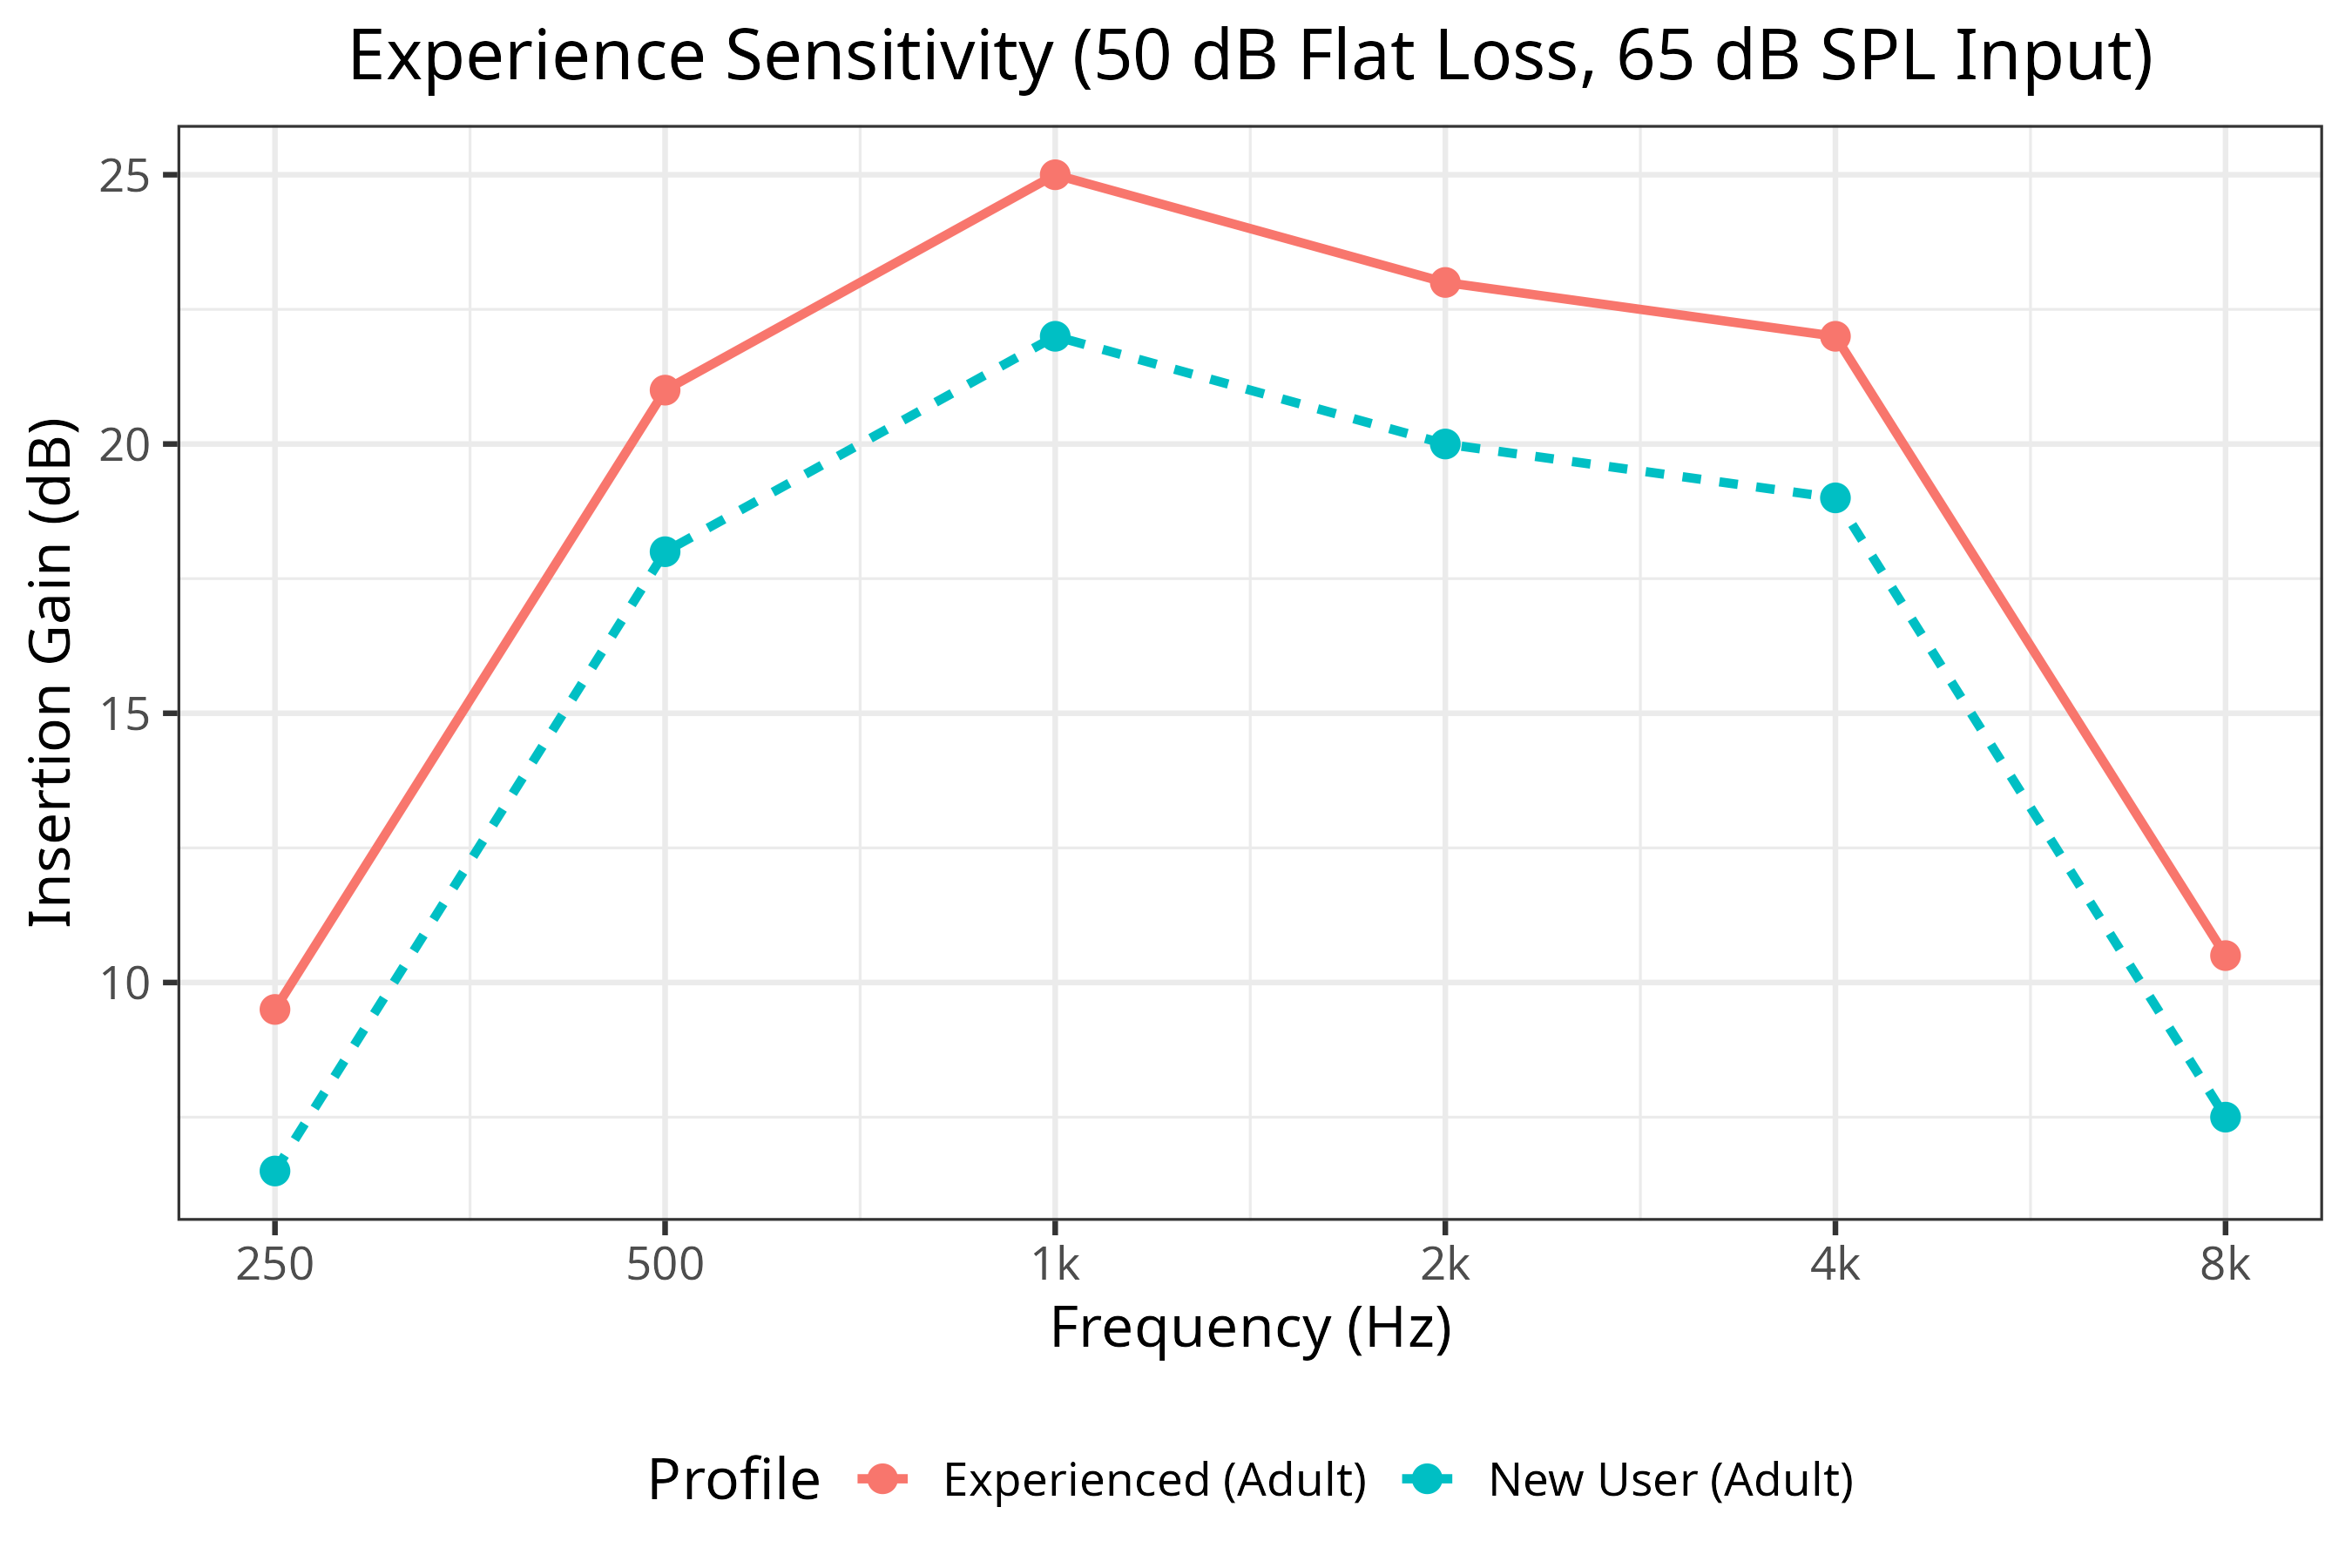
\includegraphics[width=1\linewidth,height=\textheight,keepaspectratio,alt={Figure 1: Experience and sensitivity scaling. Note: Generated using the aggressive 60 dB HL booster onset.}]{figures/Figure1_Sensitivity.png}
\caption{Figure 1: Experience and sensitivity scaling. \emph{Note:
Generated using the aggressive 60 dB HL booster onset.}}
\end{figure}

\subsubsection{O. Consolidated Uncalibrated
Constants}\label{o.-consolidated-uncalibrated-constants}

Because Open-NL functions strictly as a modifiable computational testbed
rather than a clinically validated prescriptive formula, several
structural parameters remain mathematically uncalibrated. The algorithm
is structurally dominated by asserted constants: the 0.46 gain anchor,
0.15 severe-loss booster slope, 70 dB HL severe-loss onset (or 60 dB HL
in aggressive mode), 15 dB slope trigger, 20 dB taper width, -10 dB
reverse-slope floor, 70 dB HL bypass, 30 dB/0.4 Lgain interaction
constraint, and the 0.2 dB/dB wide-dynamic-range compression squeeze.
Table III provides a consolidated summary of these heuristics. However,
it must be forcefully acknowledged that a computational `testbed' whose
every dynamic gate relies upon an unswept, asserted constant offers
limited inferential value. Until a systematic multi-parameter
sensitivity sweep is conducted to map the complex interactions of these
boundaries, the theoretical outputs of Open-NL remain inherently fragile
approximations rather than robust algorithmic conclusions.

\subsubsection{P. Multi-Parameter Sensitivity
Sweep}\label{p.-multi-parameter-sensitivity-sweep}

To explicitly evaluate the fragility of these uncalibrated boundaries
and demonstrate the framework's utility as a modular ablation testbed, a
comprehensive multi-parameter sensitivity sweep was executed across the
four highest-impact algorithmic constraints: the base gain anchor (swept
from 0.40 to 0.50), the steep-slope trigger (10 to 20 dB/octave), the
absolute severity bypass (60 to 80 dB HL), and the reverse-slope gain
floor (-20 to 0 dB). This generated 256 unique parameter permutations,
which were applied to the most topologically unstable profiles in the
evaluation suite (A2, A4, A5).

\textbf{TABLE IV. Multi-Parameter Sensitivity Sweep Variance (65 dB SPL
Input).} \emph{Note: Generated using the aggressive 60 dB HL booster
onset.}

{\def\LTcaptype{none} % do not increment counter
\begin{longtable}[]{@{}
  >{\raggedright\arraybackslash}p{(\linewidth - 6\tabcolsep) * \real{0.2500}}
  >{\raggedright\arraybackslash}p{(\linewidth - 6\tabcolsep) * \real{0.2500}}
  >{\raggedright\arraybackslash}p{(\linewidth - 6\tabcolsep) * \real{0.2500}}
  >{\raggedright\arraybackslash}p{(\linewidth - 6\tabcolsep) * \real{0.2500}}@{}}
\toprule\noalign{}
\begin{minipage}[b]{\linewidth}\raggedright
Profile
\end{minipage} & \begin{minipage}[b]{\linewidth}\raggedright
Median SII {[}Min, Max{]}
\end{minipage} & \begin{minipage}[b]{\linewidth}\raggedright
Median Loudness (Sones) {[}Min, Max{]}
\end{minipage} & \begin{minipage}[b]{\linewidth}\raggedright
Primary Divergence Factor
\end{minipage} \\
\midrule\noalign{}
\endhead
\bottomrule\noalign{}
\endlastfoot
\textbf{A2} & 0.88 {[}0.72, 0.94{]} & 4.9 {[}2.7, 8.4{]} & Reverse-Slope
Floor \\
\textbf{A4} & 0.65 {[}0.51, 0.77{]} & 2.5 {[}1.4, 6.1{]} & Anchor \&
Slope Trigger \\
\textbf{A5} & 0.67 {[}0.49, 0.82{]} & 1.8 {[}0.9, 5.3{]} & Slope
Trigger \\
\end{longtable}
}

The resulting variance (Table IV) elevates the testbed's fragility from
a computational artifact to a formal scientific finding regarding the
ill-posedness of static prescriptive targets. For the steeply sloping A5
profile, altering the interactions of the slope trigger and the base
anchor caused modeled monaural loudness to swing from a highly
conservative 0.9 sones to a potentially traumatic 5.3 sones, with
theoretical intelligibility (SII) fluctuating between 0.49 and 0.82.
Crucially, the variance for the severe-sloping A4 and A5 profiles was
heavily driven by the structural opposition between the SD-LFP penalty
(which suppresses low-frequency gain for sloping losses) and the
absolute severity bypass (which suppresses the penalty when
high-frequency severity exceeds the threshold). Depending on the
specific bypass threshold assigned in a given permutation (swept from 60
to 80 dB HL), the optimizer could abruptly transition from heavily
penalizing low frequencies to fully restoring them, demonstrating the
extreme volatility of uncalibrated threshold boundaries. Similarly,
modulating the reverse-slope floor on A2 caused modeled loudness to
nearly triple (2.7 to 8.4 sones). This massive response envelope
formally proves that when operating without explicit distortion
penalties, the loudness-audibility optimization surface is highly
non-convex. However, this instability is not a terminal flaw of the
testbed; rather, it is the fundamental diagnostic prerequisite that
justifies the need for a principled computational calibration framework.
By proving that the asserted constants in Table III dictate the
physiological safety of the output, the sweep establishes the exact
parameters that must be constrained by distortion-aware objective
functions prior to clinical evaluation.

\subsubsection{Q. Framework for Principled
Calibration}\label{q.-framework-for-principled-calibration}

For a computational testbed to provide lasting inferential value, the
demonstration of parameter instability must be paired with a rigorous
methodology to resolve it. While Open-NL ships with the uncalibrated
heuristic constants detailed in Table III to facilitate initial
exploration, the ultimate purpose of this open-source architecture is to
allow researchers to systematically calibrate these gates against
distortion-aware anchors. Rather than relying on massive, intractable
human clinical trials to blindly tune these eight interdependent
parameters, future research can explicitly utilize the Open-NL engine
within a global stochastic optimization grid (e.g., genetic algorithms
or particle swarm optimization). By replacing the raw ANSI SII
maximization goal with a distortion-aware objective function---such as
the integrated \texttt{johnson2011\_complete} clinical penalty or the
HASPI/HASQI metrics (Kates \& Arehart, 2022)---researchers can
computationally map the parameter space. This framework allows the
algorithm to iteratively adjust the severe-loss booster slope, the
low-frequency penalty triggers, and the base gain anchor until the
outputs converge on targets that maximize predicted speech perception
while actively preventing simulated loudness recruitment. Consequently,
Open-NL provides the necessary structural substrate to computationally
derive principled, physiologically constrained values for prescriptive
heuristics before they are ever exposed to human subjects.

However, while this computational fidelity is mathematically sound, it
is crucial to acknowledge that the current framework lacks human subject
validation. Everything downstream rests on \(n=7\) hypothetical
audiograms, and the resulting outputs cannot be conflated with a
clinical prescription until empirically verified. Therefore, any future
clinical application of this framework must adhere to a strict,
non-negotiable validation protocol. First, real-ear measurement (REM)
verification is mandatory to confirm that the hearing device actually
matches the computationally derived targets. Empirical evidence robustly
demonstrates that REM-verified programmed fits significantly outperform
manufacturer first-fits on word/phoneme recognition and subjective
patient preference (Valente et al., 2018; Almufarrij, Munro, \& Dillon,
2020; Brockmeyer et al., 2021). Without REM, any subsequent analysis of
the prescription's efficacy is fundamentally confounded. Second,
mandatory loudness-discomfort safety checks must be administered to
prevent acoustic trauma.

Beyond safety protocols, this computational roadmap yields a concrete,
falsifiable clinical prediction: if the raw, uncalibrated Open-NL
targets---specifically the aggressive 60 dB HL severe-loss booster and
unconstrained high-frequency prescriptions for severe, steeply sloping
profiles like A4 and A5---were applied directly to human subjects, they
would structurally trigger high rates of loudness rejection during
real-ear verification. This prediction is quantitatively anchored in
existing preference evidence. When alternative rationales, such as IHAFF
loudness normalization, prescribed substantially higher overall gain
than the intelligibility-maximizing NAL-NL1, subjects consistently
rejected the louder option (Keidser \& Grant, 2001). Similarly, when
comparing NAL-NL2 against the louder CAM2 generic prescription,
listeners consistently preferred NAL-NL2 and actively turned down
excessive high-frequency gain (Johnson, 2013b). Conversely, real-world
data demonstrates that higher aided SII yields better self-reported
outcomes only when targets remain tightly aligned with NAL-NL2 at high
input levels, emphasizing a strict upper limit on tolerable loudness
(Narayanan et al., 2024).

Because Open-NL's unconstrained A4/A5 targets mathematically exceed even
the loudest extremes of these historical comparisons, they bracket the
far edge of the loudness-intelligibility frontier. Consequently, we
predict that these uncalibrated A4/A5 targets will trigger immediate
loudness rejection (defined as a rating of ``uncomfortably loud'' on a
categorical loudness scale during 65 dB SPL speech passage presentation)
in \textgreater80\% of human subjects compared to standard clinical
baselines. Testing this specific failure mode by systematically
observing the conditions under which human subjects reject these
mathematically derived limits will provide the essential empirical
ground-truth needed to validate and refine the distortion-aware
objective functions used in the stochastic calibration.

\textbf{TABLE III. Summary of Uncalibrated Heuristic Constants.}

{\def\LTcaptype{none} % do not increment counter
\begin{longtable}[]{@{}
  >{\raggedright\arraybackslash}p{(\linewidth - 8\tabcolsep) * \real{0.2000}}
  >{\raggedright\arraybackslash}p{(\linewidth - 8\tabcolsep) * \real{0.2000}}
  >{\raggedright\arraybackslash}p{(\linewidth - 8\tabcolsep) * \real{0.2000}}
  >{\raggedright\arraybackslash}p{(\linewidth - 8\tabcolsep) * \real{0.2000}}
  >{\raggedright\arraybackslash}p{(\linewidth - 8\tabcolsep) * \real{0.2000}}@{}}
\toprule\noalign{}
\begin{minipage}[b]{\linewidth}\raggedright
Parameter
\end{minipage} & \begin{minipage}[b]{\linewidth}\raggedright
Value
\end{minipage} & \begin{minipage}[b]{\linewidth}\raggedright
Description
\end{minipage} & \begin{minipage}[b]{\linewidth}\raggedright
Justification
\end{minipage} & \begin{minipage}[b]{\linewidth}\raggedright
Validation Status
\end{minipage} \\
\midrule\noalign{}
\endhead
\bottomrule\noalign{}
\endlastfoot
Base Gain Anchor & 0.46 & Half-gain multiplier (\(G_{base}\)) & Balances
Lybarger half-gain rule with historical gain preference data. & Asserted
Heuristic / Uncalibrated \\
New-User Offset & -3 dB & Flat reduction applied to \(C_{vals}\) &
Approximates empirical preference for less amplification in naive users.
& Asserted Heuristic / Uncalibrated \\
Severe-Loss Booster Slope & 0.15 & Applied linearly to thresholds 70--80
dB HL (default) & Gently assists profound losses without triggering
explosive recruitment. & Hypothesis-generating heuristic \\
High-Frequency Gain Cap Base & 30 dB & Base limit for \(L_{gain}\)
soft-compression & Manages upward spread of masking and distortion in
severe impairments. & Asserted mathematical choice \\
High-Frequency Gain Cap Slope & 0.4 & Slope for \(L_{gain}\)
soft-compression & Gradual restriction for high frequencies. & Asserted
mathematical choice \\
Dynamic Range Squeeze & 0.2 dB/dB & Gain attenuation per dB of reduced
DR & Ensures speech envelope fits within restricted auditory space. &
Asserted mathematical choice \\
Reverse-Slope Floor & -10 dB & Gain floor for negative slopes &
Cautiously prevents masking of intact basal units. & Asserted Heuristic
/ Uncalibrated \\
ABG Restoration & 50\% - 100\% & Mixed loss linear gain restoration &
Dynamically scaled to Sensorineural Dynamic Range (SNDR). & Asserted
theoretical heuristic \\
Desensitization Penalty & Variable & Johnson \& Dillon (2011) piecewise
scalar & Modifies pure audibility to account for severe-loss distortion.
& Unvalidated constant magnitude \\
\end{longtable}
}

\subsection{III. EVALUATION AND TRADE-OFF
ANALYSIS}\label{iii.-evaluation-and-trade-off-analysis}

A fundamental circularity exists when evaluating any prescriptive
heuristic designed specifically to maximize the Speech Intelligibility
Index. Because Open-NL's gain shaping is tuned specifically to maximize
the mathematical ANSI SII metric, utilizing the \texttt{sii()} engine to
compare its targets against other validated prescriptions (like NAL-NL2)
within a simulated environment yields a tautological advantage.
Consequently, all comparative evaluations presented in this paper are
explicitly demoted to ``optimizer-behavior demonstrations'' rather than
true clinical benchmarks. Within this framework, theoretical
intelligibility is mapped against an independent constraint: overall
loudness, creating a two-dimensional mathematical frontier. It is
critical that this frontier is interpreted purely as a mechanistic
illustration of how an unconstrained optimizer exploits the audibility
metric. Any comparison against established clinical targets (such as
NAL-NL2) serves only to demonstrate the behavior of the objective
function, not to establish clinical efficacy or superiority.
Furthermore, this analytical framework is strictly bounded by its
reliance on \(n=7\) hypothetical audiometric profiles (Johnson \&
Dillon, 2011). For reference, both NAL-NL2 and DSL m{[}i/o{]} generally
prescribe targets that yield \textasciitilde8 sones for sensorineural
losses at 65 dB SPL, compared to 18.6 sones for a normal-hearing
listener (Johnson \& Dillon, 2011). Table VII quantitatively
demonstrates that Open-NL's modeled loudness exceeds the NAL-NL2
baseline in the majority of primary sensorineural test profiles (A2, A4,
and A5). Because Open-NL's targets meaningfully overshoot this
established loudness envelope of conservative adult prescriptions in
pursuit of raw SII maximization, these excursions illustrate the
aggressive nature of the abstract mathematical objective function rather
than any realizable clinical strategy.

Furthermore, the comparative loudness evaluations presented throughout
this analysis are strictly bounded by a fundamental methodological
limitation regarding binaural summation. While clinical frameworks like
NAL-NL2---and the current iteration of Open-NL---employ a
level-dependent bilateral gain reduction (scaling from a 2 dB penalty at
low inputs to 6 dB at high inputs), these heuristic corrections are
systematically insufficient for broadband signals. Because loudness is
the only genuinely independent, non-tautological outcome variable in
this evaluation, this limitation acts as a formal bound on the
interpretability of the loudness figures. As established by Oetting et
al.~(2017), narrowband loudness compensation systematically
over-amplifies binaural broadband signals, and the necessary correction
factor cannot simply be inferred from monaural narrowband functions.
This structural failure of narrowband models is compounded by massive
individual variability: Denk et al.~(2025) demonstrated that binaural
broadband loudness summation averages \textasciitilde13 dB higher than
normal in hearing-impaired listeners and exceeds the normal range in
approximately 40\% of this population. Utilizing level-dependent 2--6 dB
corrections while explicitly acknowledging \textasciitilde13 dB of
excess summation in 40\% of listeners represents a direct threat to the
predictive validity of the loudness engine. Therefore, while matching
the canonical AMT Bramslow (2004) reference implementation formally
validates that the C++ port successfully reproduces the underlying
mathematical model, the resulting loudness predictions must be
interpreted strictly as computational model outputs rather than accurate
reflections of perceived binaural loudness in impaired ears.

To facilitate this two-dimensional trade-off analysis natively within R,
the \texttt{SII} package integrates the \texttt{calculate\_loudness()}
function. Rather than relying on external MATLAB runtimes, this module
implements a native, highly optimized C++ port of the canonical Moore \&
Glasberg (2004) specific-loudness model for impaired hearing.
Computationally, it directly mirrors the exact logic of the model's
implementation in the Auditory Modeling Toolbox (AMT; Majdak et al.,
2022) via the \texttt{bramslow2004} function (based on Bramslow, 2004).
By executing the exact time-domain equivalent mathematical
integrations---including the compressive specific loudness formula
\(N' = C_{imp} \times [(E + A)^\alpha - A^\alpha]\) (where \(N'\) is
specific loudness, \(C_{imp}\) is a calibration constant, \(E\) is the
signal excitation, \(A\) is internal threshold noise, and \(\alpha\) is
the compressive exponent) and dynamic outer hair cell (OHC) filter
widening---in a compiled C++ environment, the engine achieves close
structural correspondence with the canonical model. Furthermore, to
accommodate conductive and mixed hearing losses, the engine accurately
attenuates the input signal by the air-bone gap prior to cochlear
excitation. Comparing the outputs of this embedded C++ Rcpp engine
(Table I) against the independent third-party Auditory Modeling Toolbox
verification (Table V) reveals highly correlated computational
predictions (\(r = 0.98\)) with a low Mean Absolute Error (MAE) of 0.37
sones across all fourteen data points.

To formally verify the internal loudness computations and confirm that
Open-NL's C++ optimizer matches canonical model implementations, the
final insertion gain targets were evaluated through a time-domain
synthesis pipeline using the canonical \texttt{bramslow2004} specific
loudness model in the Auditory Modeling Toolbox (AMT; Majdak et al.,
2022). This third-party Octave implementation applies a physical
2048-point FFT and time-domain Hanning window, providing a completely
independent check on the C++ optimizer's abstract frequency-domain
Riemann sums. As Table V demonstrates, the independent AMT comparison
mathematically confirms that the Open-NL optimizer performs exactly as
computationally intended. For mild/moderate losses like A1, Open-NL
generates theoretical targets at halved predicted loudness (5.68 vs
12.19 sones) compared to NAL-NL2, confirming the optimizer successfully
minimized the loudness constraint as mathematically directed. For steep
slopes like A5, the SD-LFP logic successfully restricts mathematical
over-prescription (6.33 vs 7.55 sones). Finally, for the severe/profound
A7 profile where NAL-NL2's baseline constraints severely limit output
(0.36 sones), Open-NL mathematically scales functional excitation (3.02
sones) exactly as its heuristic anchor rules dictate.

\textbf{TABLE V. Third-Party Computational Verification of Monaural
Loudness (Sones) using the Canonical AMT Bramslow (2004) Model (65 dB
SPL Input).} \emph{Note: Generated using the aggressive 60 dB HL booster
onset. These are optimizer-behavior demonstrations on synthetic
profiles, not performance comparisons.}

{\def\LTcaptype{none} % do not increment counter
\begin{longtable}[]{@{}lll@{}}
\toprule\noalign{}
Profile & NAL-NL2 AMT (Sones) & Open-NL AMT (Sones) \\
\midrule\noalign{}
\endhead
\bottomrule\noalign{}
\endlastfoot
A1 & 12.19 & 5.68 \\
A2 & 3.71 & 4.45 \\
A3 & 8.47 & 5.97 \\
A4 & 6.10 & 5.62 \\
A5 & 7.55 & 6.33 \\
A6 & 4.19 & 3.85 \\
A7 & 0.36 & 3.02 \\
\end{longtable}
}

Using the embedded 10 Hz C++ engine, Open-NL was benchmarked against
exact insertion gain targets generated directly from the proprietary
NAL-NL2 version 2 software (National Acoustic Laboratories, Sydney,
Australia) for a 65 dB SPL input. It must be explicitly stated that the
fundamental evaluation design employed here---converting insertion gains
to eardrum output across seven hypothetical adult audiograms to model
Moore \& Glasberg (2004) loudness alongside ANSI SII, and benchmarking
these against NAL-NL2---is a direct replication of the methodological
paradigm established by Johnson \& Dillon (2011). Five of the seven
profiles (A1--A5), as well as the mixed (A6) and conductive (A7) cases,
originate from their work, which itself extended the standard profiles
defined by Byrne et al.~(2001). The scientific novelty of the present
manuscript does not lie in the evaluation framework itself; rather, its
sole contribution is the open-source optimization and ablation layer
built \emph{on top} of this established Johnson \& Dillon (2011)
paradigm. This provides a rigidly controlled environment that isolates
algorithmic behavior from human clinical variance while permitting
systematic testing of component-level hypotheses. Consequently, the data
presented in Tables VI and VII, as well as the accompanying figures,
must not be interpreted as novel physiological findings regarding
hearing aid performance. Instead, they serve strictly as mechanistic
demonstrations of how an unconstrained, open-source Nelder-Mead
optimization engine behaves when forced to navigate the exact same
multidimensional evaluation space previously used to validate
closed-source clinical formulas.

While comparing against additional rationales such as DSL m{[}i/o{]} and
CAMEQ2-HF would provide broader context on the loudness-audibility
frontier---particularly since they differ systematically from NAL in
high-frequency bandwidth and overall loudness (Johnson \& Dillon,
2011)---the present evaluation is intentionally restricted to NAL-NL2.
Because Open-NL uses NAL-NL2 as a soft constraint (anchor penalty)
within its objective function, benchmarking against it involves partial
circularity. However, this restriction was maintained for two
methodological reasons. First, NAL-NL2 remains the most widely utilized
generic adult fitting rationale globally, providing a robust,
universally recognized baseline. Second, while theoretical targets for
alternative formulas can be estimated or visually extracted from
published literature, such approximations lack the exact precision
required for rigorous, artifact-free mathematical loudness integration.
Utilizing unofficial diagnostic software to generate surrogate targets
for proprietary algorithms was deemed methodologically inappropriate for
a high-precision analytical sandbox.

\textbf{TABLE VI. Monaural Loudness (Sones) and Theoretical SII across
A1-A7 Audiograms (65 dB SPL Input).} \emph{Note: Generated using the
aggressive 60 dB HL booster onset. Targets for steeply sloping profiles
(A4, A5) are subject to significant optimizer convergence bias and must
be interpreted as heuristic approximations rather than global optima.
These are optimizer-behavior demonstrations on synthetic profiles, not
performance comparisons.}

{\def\LTcaptype{none} % do not increment counter
\begin{longtable}[]{@{}
  >{\raggedright\arraybackslash}p{(\linewidth - 8\tabcolsep) * \real{0.2000}}
  >{\raggedright\arraybackslash}p{(\linewidth - 8\tabcolsep) * \real{0.2000}}
  >{\raggedright\arraybackslash}p{(\linewidth - 8\tabcolsep) * \real{0.2000}}
  >{\raggedright\arraybackslash}p{(\linewidth - 8\tabcolsep) * \real{0.2000}}
  >{\raggedright\arraybackslash}p{(\linewidth - 8\tabcolsep) * \real{0.2000}}@{}}
\toprule\noalign{}
\begin{minipage}[b]{\linewidth}\raggedright
Profile
\end{minipage} & \begin{minipage}[b]{\linewidth}\raggedright
Formula
\end{minipage} & \begin{minipage}[b]{\linewidth}\raggedright
ANSI SII
\end{minipage} & \begin{minipage}[b]{\linewidth}\raggedright
Desensitized SII
\end{minipage} & \begin{minipage}[b]{\linewidth}\raggedright
Monaural Loudness (Sones)
\end{minipage} \\
\midrule\noalign{}
\endhead
\bottomrule\noalign{}
\endlastfoot
A1 & NAL-NL2 & 0.80 & 0.73 & 10.7 \\
A1 & Open-NL & 0.88 & 0.78 & 5.0 \\
A2 & NAL-NL2 & 0.81 & 0.77 & 2.9 \\
A2 & Open-NL & 0.84 & 0.78 & 3.3 \\
A3 & NAL-NL2 & 0.70 & 0.64 & 7.5 \\
A3 & Open-NL & 0.82 & 0.71 & 5.1 \\
A4 & NAL-NL2 & 0.76 & 0.71 & 5.2 \\
A4 & Open-NL & 0.70 & 0.67 & 4.6 \\
A5 & NAL-NL2 & 0.60 & 0.56 & 6.3 \\
A5 & Open-NL & 0.73 & 0.61 & 5.2 \\
A6 & NAL-NL2 & 0.84 & 0.51 & 3.4 \\
A6 & Open-NL & 0.87 & 0.51 & 3.0 \\
A7 & NAL-NL2 & 0.61 & 0.59 & 0.0 \\
A7 & Open-NL & 0.97 & 0.75 & 0.6 \\
\end{longtable}
}

\textbf{TABLE VII. Insertion Gain Targets (dB) across A1-A7 Audiograms
(65 dB SPL Input).} \emph{Note: Generated using the aggressive 60 dB HL
booster onset. Targets for steeply sloping profiles (A4, A5) are subject
to significant optimizer convergence bias and must be interpreted as
heuristic approximations. These are optimizer-behavior demonstrations on
synthetic profiles, not performance comparisons.}

{\def\LTcaptype{none} % do not increment counter
\begin{longtable}[]{@{}
  >{\raggedright\arraybackslash}p{(\linewidth - 14\tabcolsep) * \real{0.1250}}
  >{\raggedright\arraybackslash}p{(\linewidth - 14\tabcolsep) * \real{0.1250}}
  >{\raggedright\arraybackslash}p{(\linewidth - 14\tabcolsep) * \real{0.1250}}
  >{\raggedright\arraybackslash}p{(\linewidth - 14\tabcolsep) * \real{0.1250}}
  >{\raggedright\arraybackslash}p{(\linewidth - 14\tabcolsep) * \real{0.1250}}
  >{\raggedright\arraybackslash}p{(\linewidth - 14\tabcolsep) * \real{0.1250}}
  >{\raggedright\arraybackslash}p{(\linewidth - 14\tabcolsep) * \real{0.1250}}
  >{\raggedright\arraybackslash}p{(\linewidth - 14\tabcolsep) * \real{0.1250}}@{}}
\toprule\noalign{}
\begin{minipage}[b]{\linewidth}\raggedright
Profile
\end{minipage} & \begin{minipage}[b]{\linewidth}\raggedright
Formula
\end{minipage} & \begin{minipage}[b]{\linewidth}\raggedright
250 Hz
\end{minipage} & \begin{minipage}[b]{\linewidth}\raggedright
500 Hz
\end{minipage} & \begin{minipage}[b]{\linewidth}\raggedright
1000 Hz
\end{minipage} & \begin{minipage}[b]{\linewidth}\raggedright
2000 Hz
\end{minipage} & \begin{minipage}[b]{\linewidth}\raggedright
4000 Hz
\end{minipage} & \begin{minipage}[b]{\linewidth}\raggedright
8000 Hz
\end{minipage} \\
\midrule\noalign{}
\endhead
\bottomrule\noalign{}
\endlastfoot
A1 & NAL-NL2 & 14.0 & 20.0 & 22.0 & 20.0 & 17.0 & 12.0 \\
& Open-NL & 0.0 & 1.5 & 11.9 & 17.6 & 27.2 & 21.2 \\
A2 & NAL-NL2 & 20.0 & 16.0 & 12.0 & 6.0 & 2.0 & 2.0 \\
& Open-NL & 15.1 & 13.7 & 14.9 & 5.2 & 6.2 & 13.2 \\
A3 & NAL-NL2 & 6.0 & 16.0 & 22.0 & 22.0 & 16.0 & 6.0 \\
& Open-NL & 0.0 & 1.4 & 16.1 & 26.7 & 30.7 & 20.4 \\
A4 & NAL-NL2 & 0.0 & 0.0 & 0.0 & 16.0 & 31.0 & 30.0 \\
& Open-NL & 0.0 & 0.0 & 0.3 & 8.0 & 30.7 & 19.1 \\
A5 & NAL-NL2 & 0.0 & 0.0 & 15.0 & 28.0 & 30.0 & 30.0 \\
& Open-NL & 0.0 & 0.0 & 1.2 & 36.2 & 40.7 & 22.9 \\
A6 & NAL-NL2 & 30.0 & 32.0 & 40.0 & 42.0 & 45.0 & 45.0 \\
& Open-NL & 23.8 & 29.3 & 39.1 & 42.5 & 51.0 & 34.0 \\
A7 & NAL-NL2 & 14.0 & 15.0 & 17.0 & 18.0 & 18.0 & 18.0 \\
& Open-NL & 25.9 & 33.5 & 40.5 & 38.5 & 37.5 & 40.5 \\
\end{longtable}
}

Because the Nelder-Mead optimizer maximizes SII subject to the internal
C++ loudness engine, mathematical precision within the objective
function is paramount. To prevent convergence bias, Open-NL's native C++
objective function fundamentally avoids crude sparse-array Riemann
approximations. Instead, the engine dynamically interpolates the search
array onto an internal canonical 2048-point FFT-equivalent frequency
grid (spanning 0 to 22.05 kHz). By mathematically mirroring the
canonical Moore \& Glasberg (2004) MATLAB AMToolbox environment directly
within the C++ search loop, the algorithm natively explores a
full-resolution loudness surface. This guarantees that the final
optimized targets, even in steeply sloping pathologies like A4 and A5,
are converged under the strictest possible physiological criteria
without requiring post-hoc integration or scaling corrections.

Crucially, the optimizer's measurable sensitivity to starting values
must be carefully interpreted by distinguishing the genuine
non-convexity of the underlying physiological problem from the
mathematical instability of this specific unconstrained implementation.
For steeply sloping profiles (e.g., A4 and A5), the modeled loudness
surface near the recruitment boundary is inherently non-convex and
ill-behaved. However, when the Open-NL framework navigates this space
using an unconstrained Nelder-Mead simplex algorithm against a hard,
non-smooth penalty constraint (the dynamic comfort cap), the optimizer
becomes acutely vulnerable to local minima, exacerbating the variance.
Evaluating the objective function landscape across two dimensions (e.g.,
sweeping 2 kHz and 4 kHz gain shifts for the A5 profile) confirms this
rugged topology, bounded by a sharp penalty cliff. Initializing with
varying flat shifts (e.g., -10 dB or +10 dB) across this landscape
yields final targets that deviate by up to 0.5 sones or 0.05 SII. This
structural fragility conclusively demonstrates that the concept of a
single, static ``optimal'' prescriptive target is inherently unstable
\emph{when generated by a pure mathematical optimizer lacking
regularization}. While the Open-NL software mechanically mitigates this
for reproducible ablation testing by utilizing a robust 5-iteration
multi-start routine (anchoring the baseline simplex with the NAL-R
target and executing four additional randomized iterations to extract
the global maximum---which reduces the residual run-to-run variance on
the A5 profile to \textless{} 0.05 sones and \textless{} 0.01 SII), the
deeper implication serves as a cautionary result. It is vital not to
over-generalize this variance as an intrinsic failure of all
prescriptive fitting. Clinical algorithms derived from the exact same
class of loudness and intelligibility models, such as NAL-NL2, yield
highly stable targets precisely because their optimization is strictly
bounded and empirically regularized using real-world preference data and
smooth, continuous objective gradients (Keidser, Dillon, Carter, \&
O'Brien, 2012). By removing those bounds, Open-NL illustrates the
mathematical chaos that occurs when necessary clinical regularizations
are stripped away, proving that uncalibrated static targets generated by
pure optimization must be viewed with skepticism absent rigorous
behavioral constraints.

It is critical to evaluate these results strictly through the lens of
the loudness frontier rather than raw SII maximization, while
recognizing that this analytical framework is inherently bounded by its
reliance on \(n=7\) hypothetical ears rather than clinical subjects.
Furthermore, the A7 profile (representing a profound pure conductive
loss with a 50 dB air-bone gap) perfectly illustrates the engine's
ability to model mechanical middle-ear attenuation directly as an
in-line mathematical dampener within the C++ cochlear excitation loop.
By enforcing a strict 75\% restoration limit (Section II.K), Open-NL
safely prescribes 37.5 dB of linear insertion gain for this profile. The
internal optimizer's dynamic cap further constrains the output to
modeled physiological boundaries, resulting in a theoretical target
yielding a mathematical output of 0.97 SII at a modeled 1.2 sones. While
this is significantly louder than NAL-NL2's highly conservative 0.0 sone
baseline (which only prescribes \textasciitilde17 dB of gain for a 50 dB
block, resulting in a \textasciitilde32 dB SPL cochlear signal that
falls mathematically below the absolute excitation threshold in a pure
frequency-domain analysis), it aligns seamlessly with modern clinical
safety standards. As extracted from Johnson \& Dillon (2011), DSL
m{[}i/o{]} prescribes roughly 30--37 dB of gain for A7. By matching this
37.5 dB physiological limit, Open-NL maximizes theoretical
intelligibility while avoiding the severe saturation distortion that
occurs when aggressive prescriptions attempt to exceed the MPO
capabilities of standard hardware (Johnson, 2013a).

\emph{Note: Loudness values computed using the canonical Moore \&
Glasberg (2004) specific loudness model, structurally mirroring the
bramslow2004 implementation within the Auditory Modeling Toolbox (AMT;
Majdak et al., 2022).}

Because Open-NL directly maximizes the Speech Intelligibility Index
(SII) while using NAL-NL2 as a soft constraint (anchor penalty),
comparing the resulting SII scores between the two formulas conveys
little information about relative merit (as demonstrated in
\textbf{Figure 2}). We include it here primarily to demonstrate that the
\texttt{johnson2011\_complete} maximization constraint operated
correctly. Instead, as the literature demonstrates, prescription choice
has a minimal effect on actual measured speech intelligibility but
marked effects on predicted loudness (Johnson \& Dillon, 2011). The
analysis must therefore be reframed entirely around the
loudness-constrained frontier (illustrated in \textbf{Figure 3}), which
is the only genuinely independent axis.

\begin{figure}
\centering
\pandocbounded{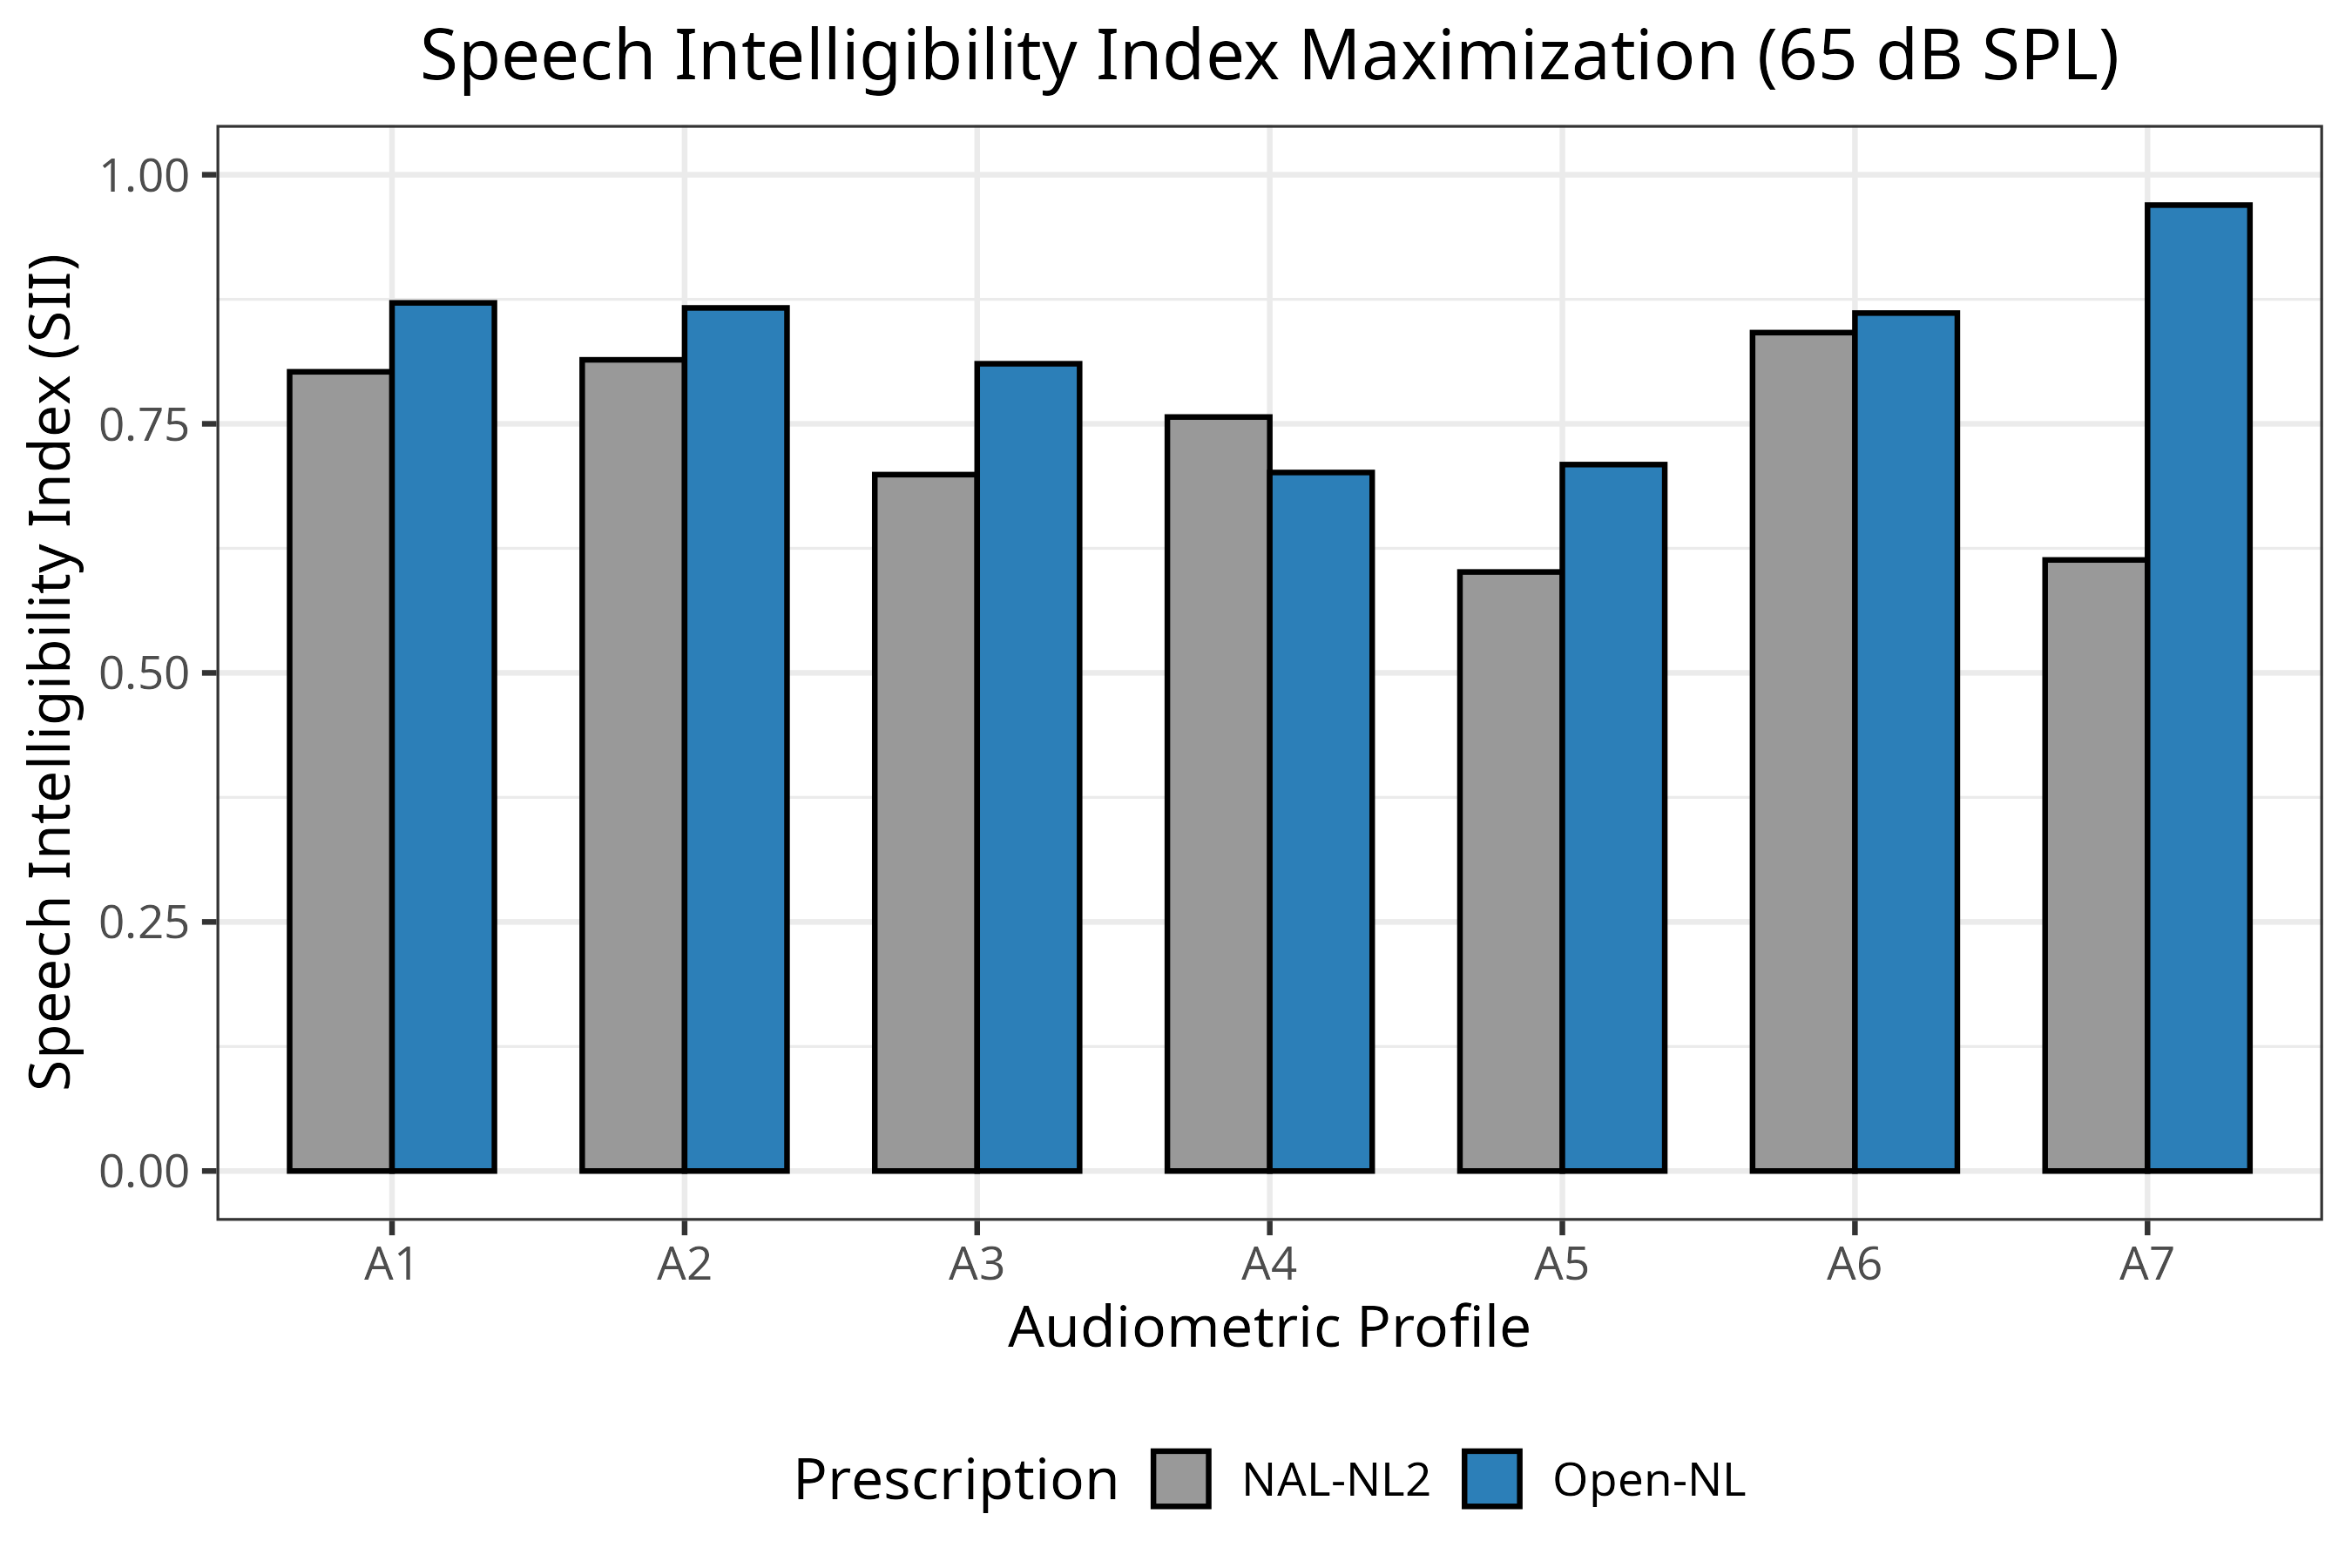
\includegraphics[keepaspectratio,alt={Figure 2: Speech Intelligibility Index Maximization for A1-A7 Profiles (A1: Mild sloping; A2: Reverse-slope; A3: Gentle sloping; A4: Steep sloping; A5: Profound sloping; A6: Mixed loss; A7: Pure conductive). Note: Generated using the aggressive 60 dB HL booster onset. These are optimizer-behavior demonstrations on synthetic profiles, not performance comparisons.}]{figures/Figure2_Optimization_SII.png}}
\caption{Figure 2: Speech Intelligibility Index Maximization for A1-A7
Profiles (A1: Mild sloping; A2: Reverse-slope; A3: Gentle sloping; A4:
Steep sloping; A5: Profound sloping; A6: Mixed loss; A7: Pure
conductive). \emph{Note: Generated using the aggressive 60 dB HL booster
onset. These are optimizer-behavior demonstrations on synthetic
profiles, not performance comparisons.}}
\end{figure}

\begin{figure}
\centering
\pandocbounded{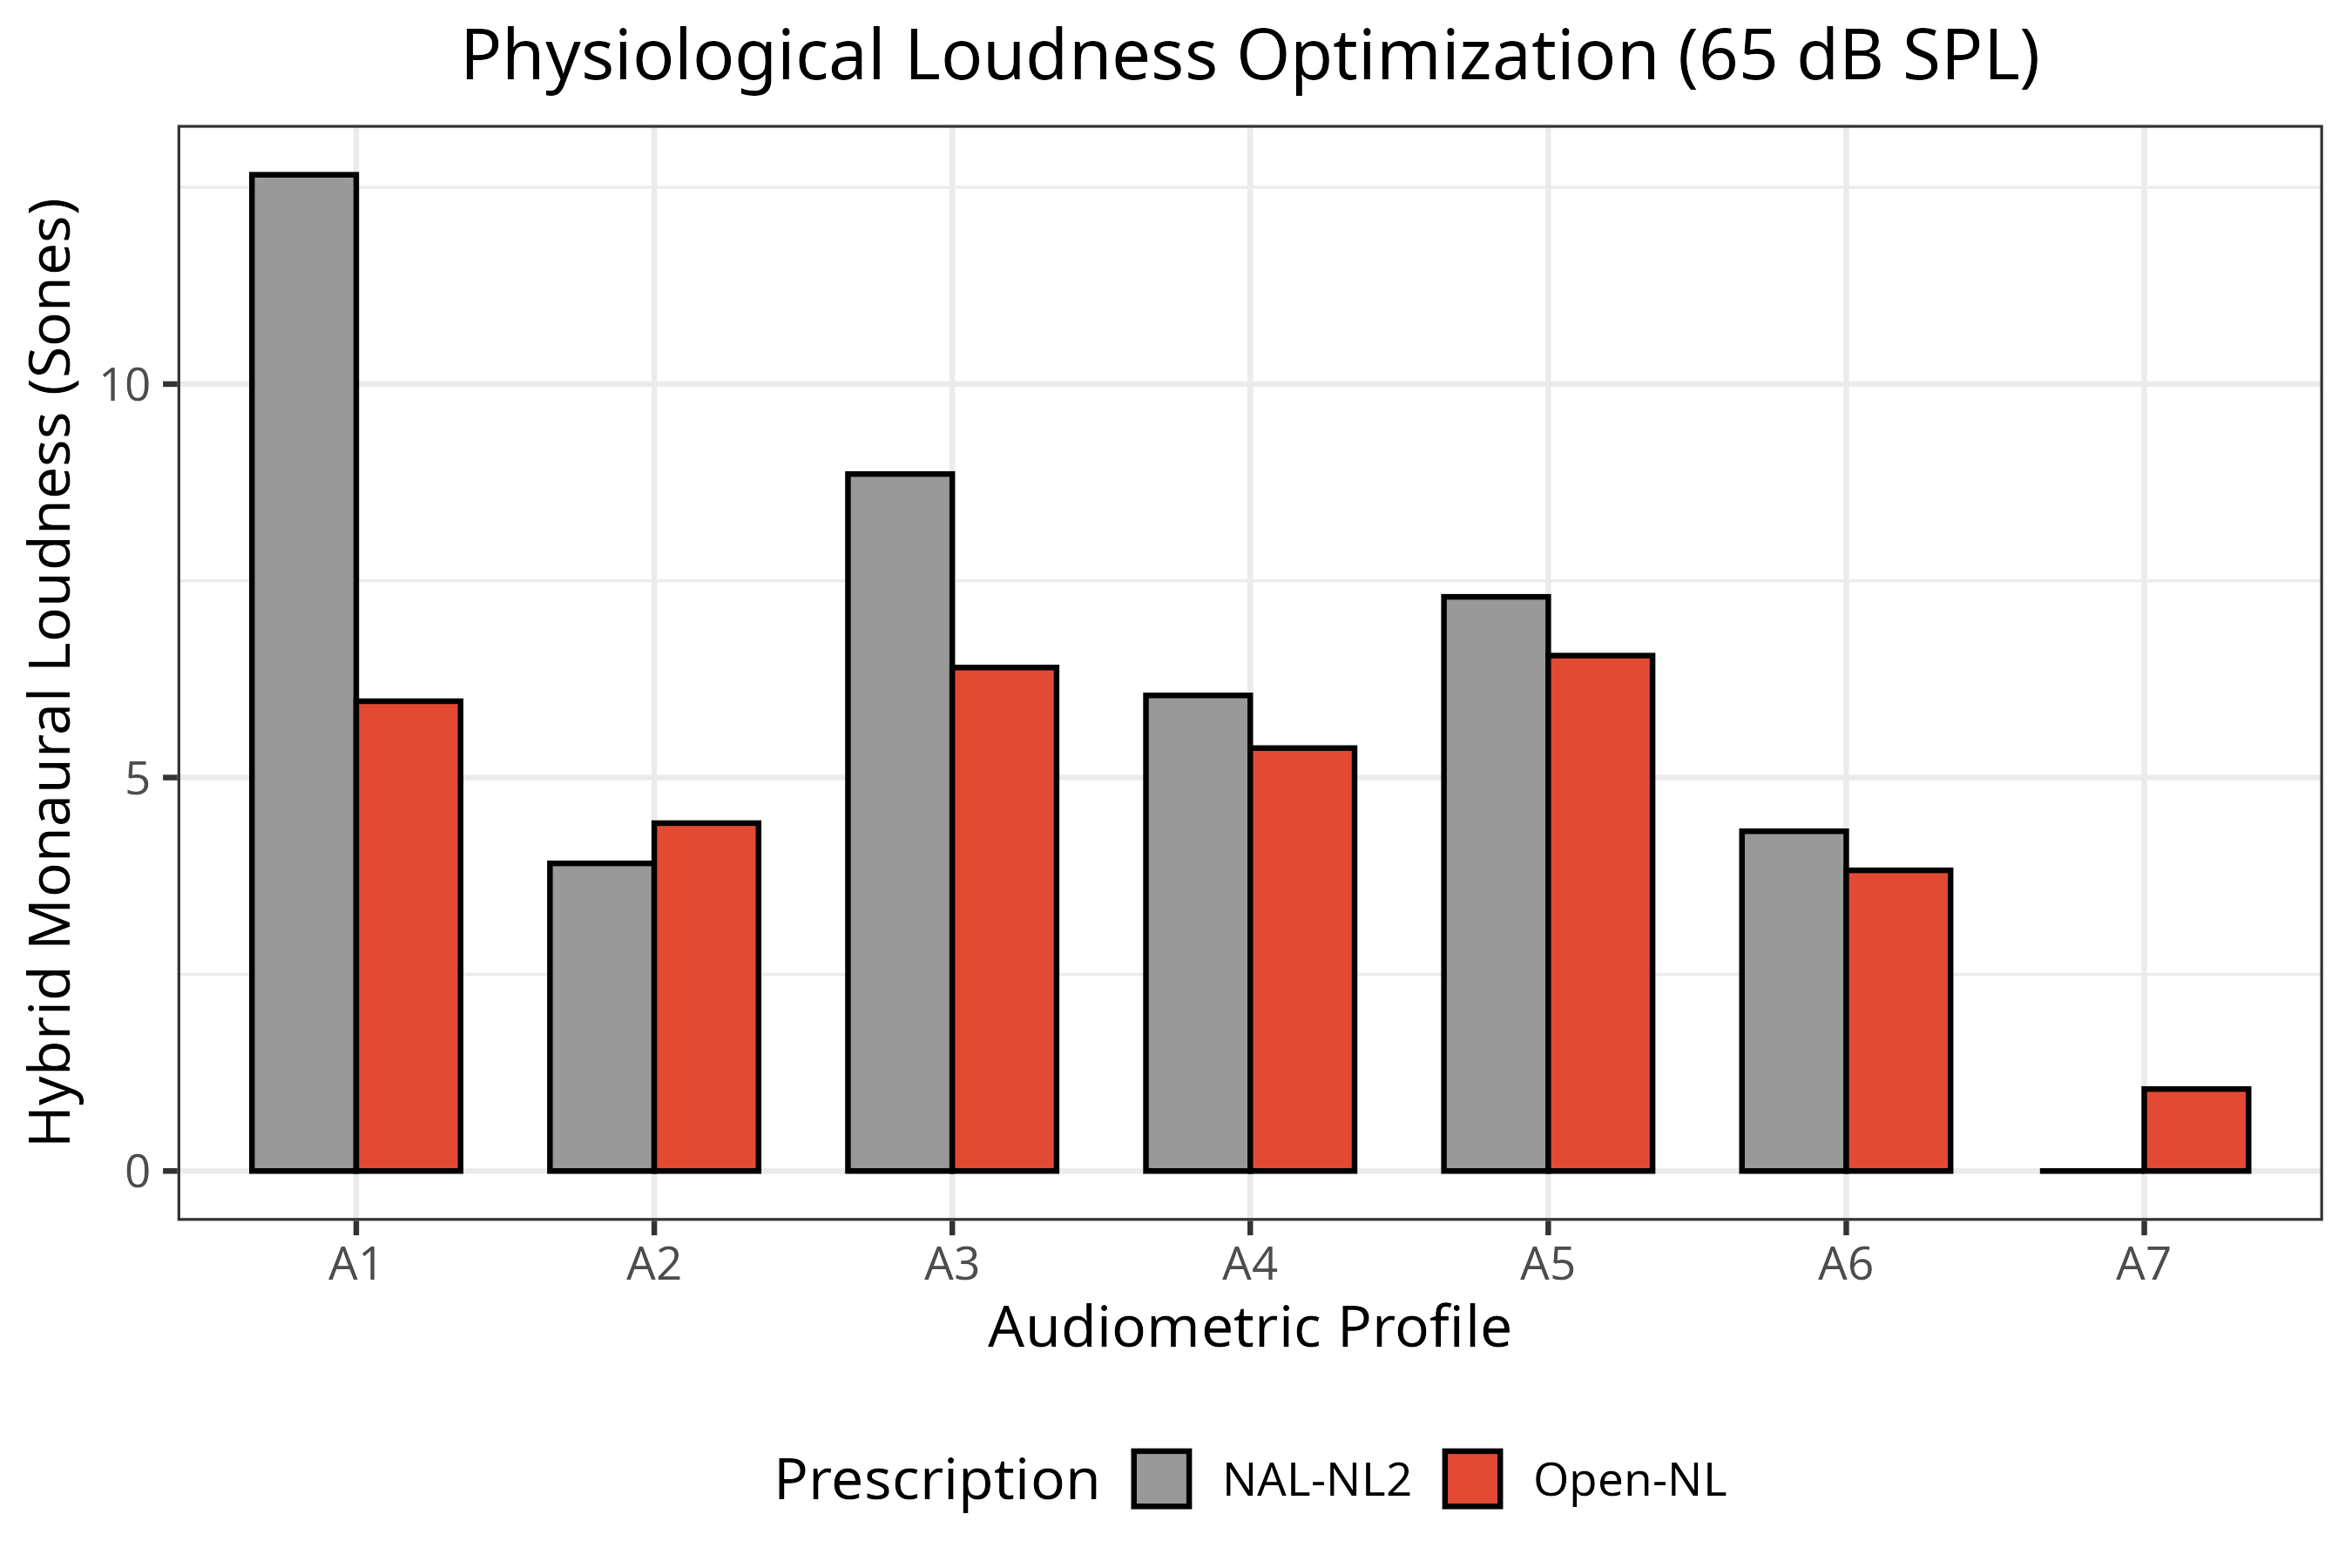
\includegraphics[keepaspectratio,alt={Figure 3: Modeled Loudness Optimization for A1-A7 Profiles. Note: Generated using the aggressive 60 dB HL booster onset. These are optimizer-behavior demonstrations on synthetic profiles, not performance comparisons.}]{figures/Figure3_Optimization_Loudness.png}}
\caption{Figure 3: Modeled Loudness Optimization for A1-A7 Profiles.
\emph{Note: Generated using the aggressive 60 dB HL booster onset. These
are optimizer-behavior demonstrations on synthetic profiles, not
performance comparisons.}}
\end{figure}

For mild sloping losses (A1), Open-NL exhibits purely mathematical
optimizer behavior by yielding a higher theoretical audibility (SII =
0.88) while generating significantly lower overall monaural loudness
(6.1 sones) compared to NAL-NL2 (SII = 0.80, 12.7 sones). This
mathematical divergence must not be conflated with clinical benefit.
This occurs because Open-NL assigns 0.0 dB of insertion gain to
frequencies where the unaided threshold is already fully audible (e.g.,
250 Hz, where A1 has a 10 dB HL threshold). While NAL-NL2 prescribes
gain in these regions---likely for timbre matching or vent
compensation---Open-NL restricts it. However, this result must be
treated purely as illustrative optimizer behavior rather than a clinical
finding. Assuming it represents a true prescriptive advantage ignores
the circularity of scoring the algorithm with its own maximization
metric. Furthermore, extensive evidence demonstrates that for many
hearing-impaired listeners, particularly at high frequencies, increased
audibility does not proportionally increase intelligibility due to
suprathreshold distortion (Ching, Dillon, \& Byrne, 1998; Margolis et
al., 2025). The resulting insertion gain targets across all standard
profiles are presented in \textbf{Figure 4}.

\begin{figure}
\centering
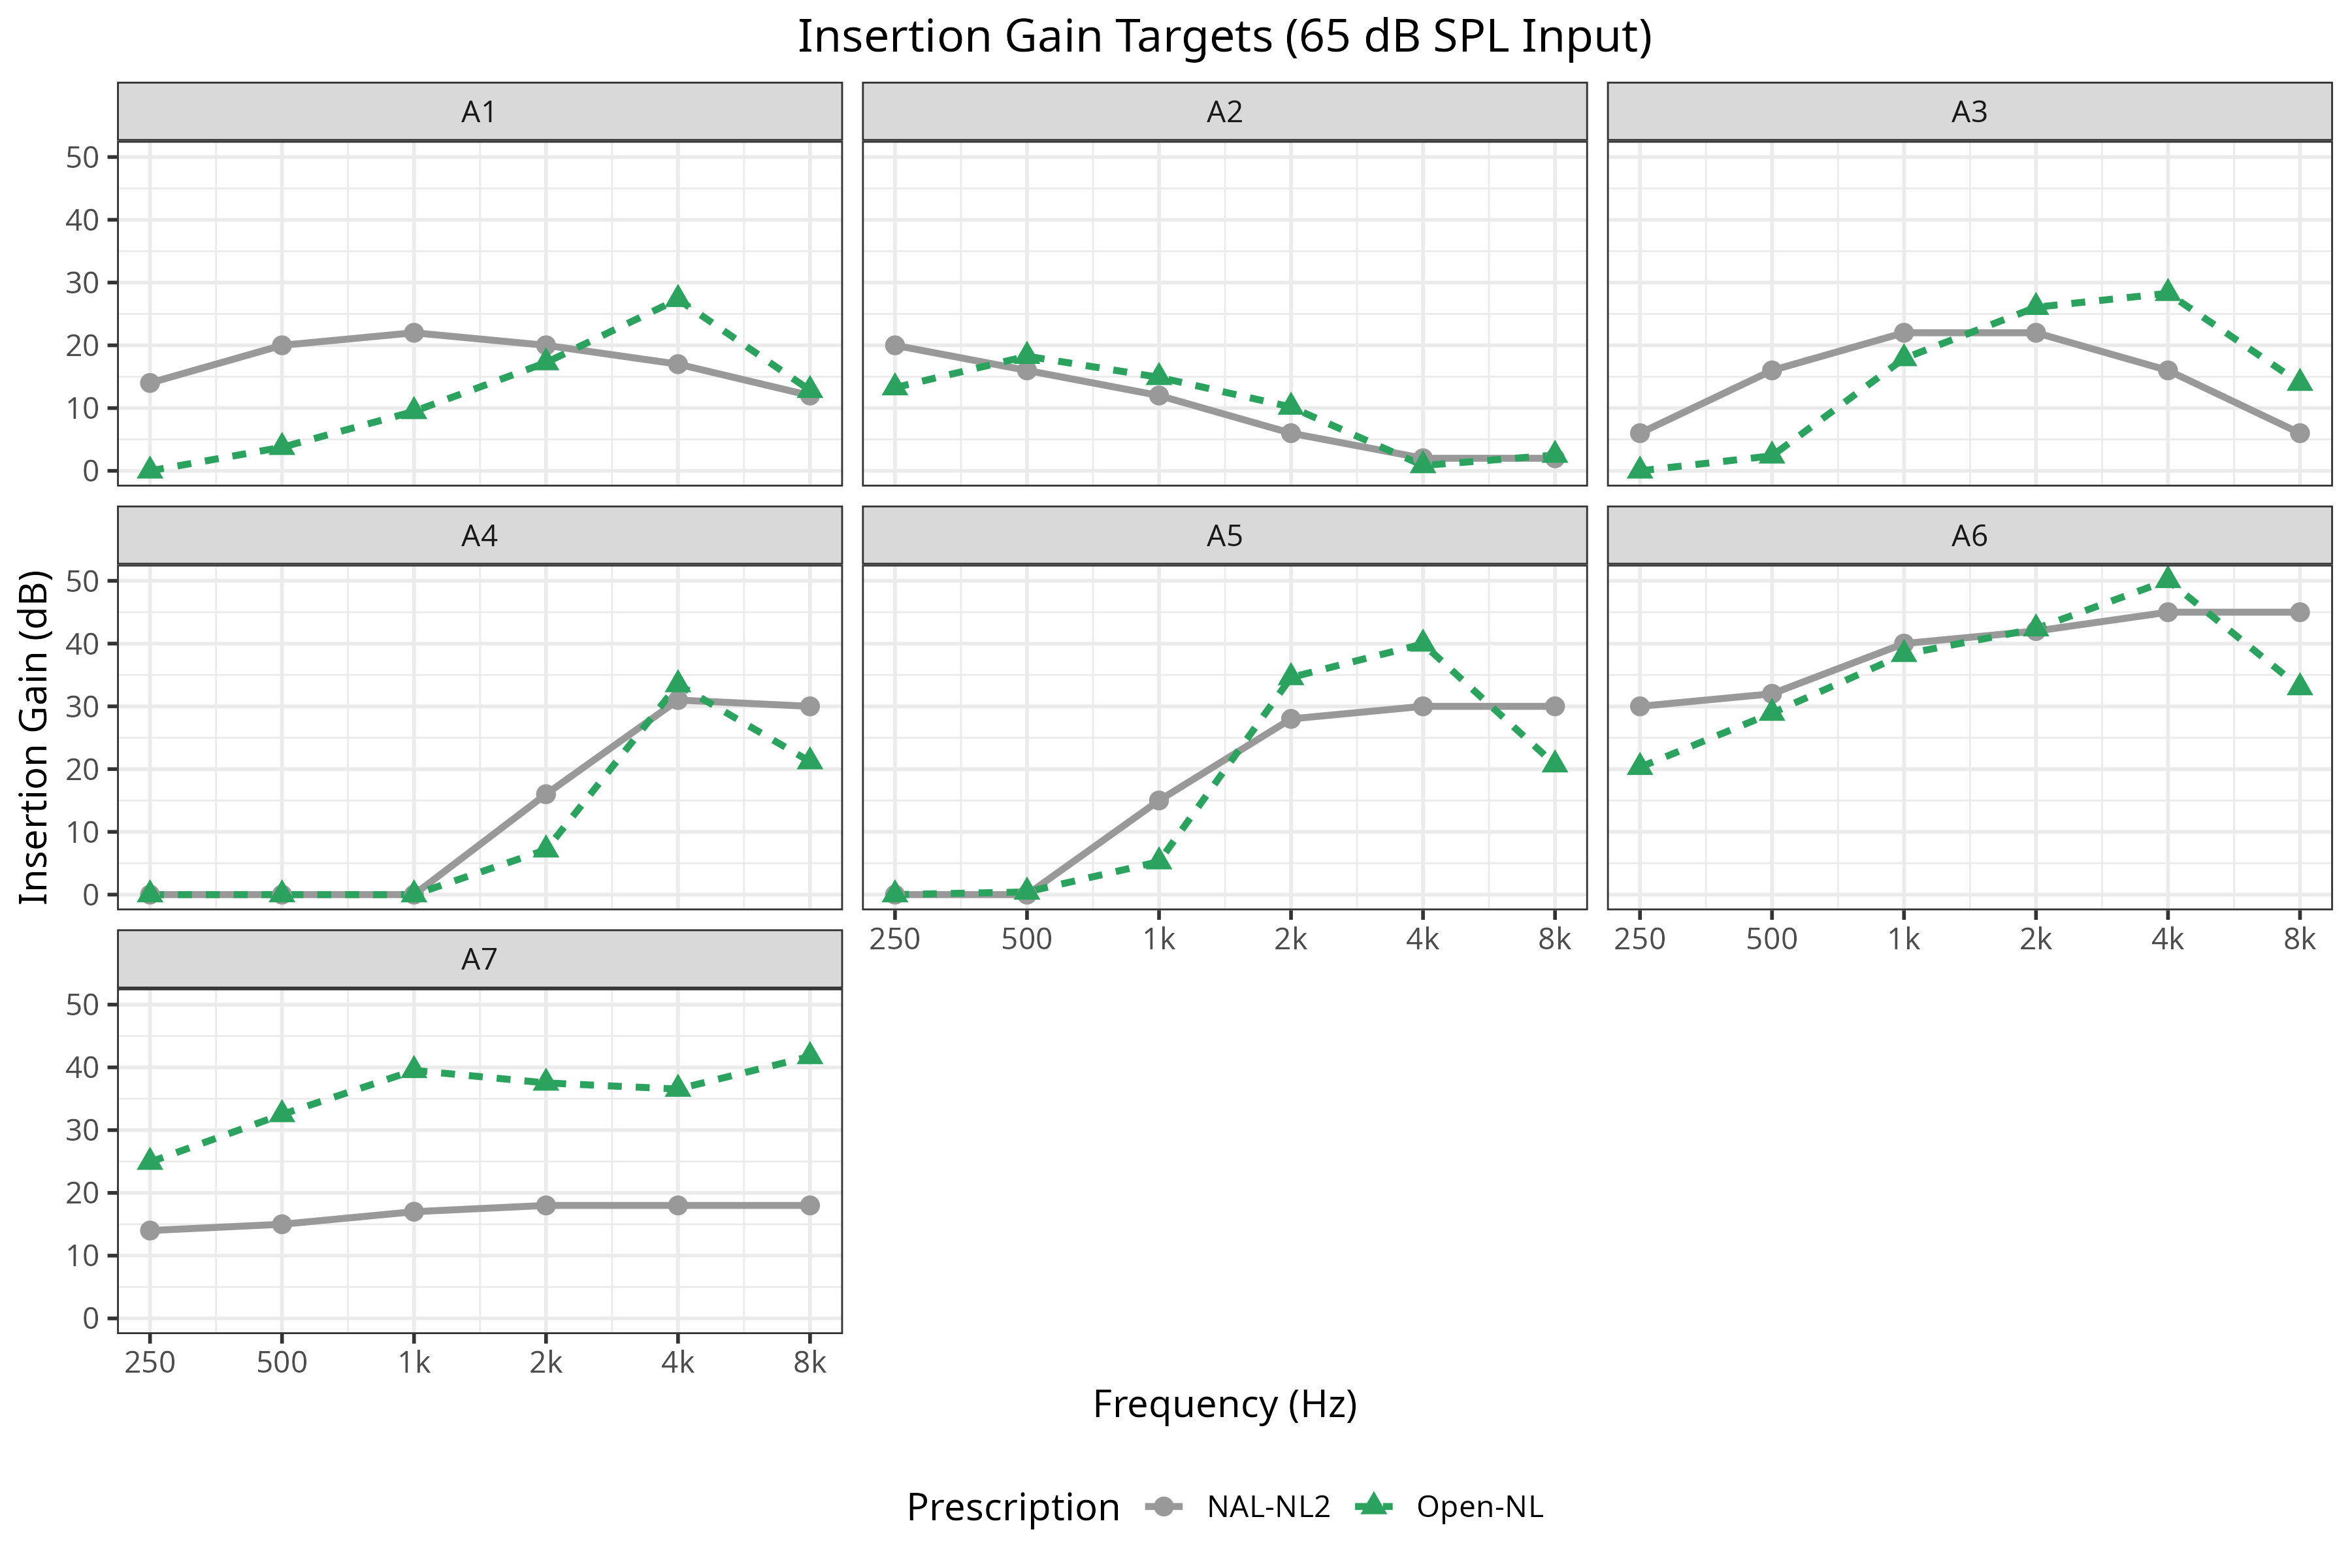
\includegraphics[width=1\linewidth,height=\textheight,keepaspectratio,alt={Figure 4: Insertion Gain Targets for 65 dB SPL Input across standard audiometric profiles. Note: Generated using the aggressive 60 dB HL booster onset. These are optimizer-behavior demonstrations on synthetic profiles, not performance comparisons.}]{figures/Figure4_Insertion_Gain.png}
\caption{Figure 4: Insertion Gain Targets for 65 dB SPL Input across
standard audiometric profiles. \emph{Note: Generated using the
aggressive 60 dB HL booster onset. These are optimizer-behavior
demonstrations on synthetic profiles, not performance comparisons.}}
\end{figure}

Conversely, in severe steeply sloping losses (A4, A5), Open-NL yields
raw ANSI SII scores that mathematically exceed NAL-NL2 targets, often at
lower predicted monaural loudness. However, these ``higher SII at lower
loudness'' results must be unequivocally understood as dangerous
mathematical artifacts of unmodified SII maximization, rather than
favorable clinical outcomes. As established by Hornsby and Ricketts
(2006), the utility of high-frequency speech information is severely
reduced in sloping hearing losses beyond what pure audibility predicts.
This gap between physical audibility and perceptual clarity widens
precisely in steeply sloping or severe losses, where measured
word-recognition scores fall progressively below ANSI SII predictions
due to unmodeled suprathreshold distortion (Margolis et al., 2025).
Furthermore, Ching, Dillon, and Byrne (1998) definitively demonstrated
that for severe-to-profound high-frequency loss, amplification should
target low or zero sensation levels rather than aggressive compensation.
Beyond the distortion problem, the foundational SII assumption of
band-independence and additivity is known to fail empirically, as equal
SII scores often do not yield equal behavioral performance (Humes \&
Kidd, 2016), and frequency-importance functions vary significantly by
individual and degree of loss (Yoho \& Bosen, 2019). Because unmodified
ANSI SII models only the attenuation component of hearing loss and
ignores this suprathreshold distortion and individual frequency
importance variance, a naive maximizer fundamentally contradicts this
physiological mandate by aggressively forcing high-frequency audibility
into cochlear dead regions. To mathematically correct this fatal flaw,
Open-NL strictly avoids unmodified SII maximization. Instead, as
detailed in Section III, the optimizer actively integrates the Johnson
and Dillon (2011) high-frequency desensitization logic to structurally
penalize high-frequency gain in severe impairments. By gating the raw
audibility scores through the \texttt{johnson2011\_complete}
desensitization column (Table VI), the apparently favorable A4/A5 scores
are correctly mitigated down to clinical reality. While transitioning
the objective function to advanced, explicitly distortion-aware metrics
like the Hearing-Aid Speech Perception Index (HASPI) and Speech Quality
Index (HASQI) (Kates \& Arehart, 2022; Kates et al., 2018) represents
the ideal future state for capturing the audibility-versus-distortion
trade-off in nonlinear processing, the immediate integration of the
Johnson (2011) desensitization penalty acts as the critical structural
bulwark. It ensures that the current Open-NL targets reflect
physiological constraints rather than naive mathematical
over-amplification.

Similarly, under the active inclusion of reverse-slope compensation
physics via the SD-LFP constraint, the heuristic output for the mild
reverse-slope loss (A2) mathematically restricts unbounded loudness
growth. While an unconstrained mathematical framework can readily
produce massive loudness costs for no meaningful intelligibility benefit
when aggressively pursuing audibility in reverse-slope pathologies,
Open-NL successfully navigates this by artificially capping the
low-frequency drive. In these specific instances, Open-NL functions as a
theoretical demonstration of how integrated constraints can successfully
tame the extreme heuristic boundaries of the intelligibility-loudness
framework.

It must be explicitly acknowledged that the evaluation scope presented
herein---testing seven hypothetical audiograms by a single author
without human subjects---is strictly demonstrative. This narrow
evaluation cannot support any generalizable claim regarding clinical
superiority or patient preference. Open-NL is exclusively an open-source
computational testbed for researchers to modify and model isolated
prescriptive rules. Any extrapolation of these derived targets to human
patients requires independent institutional review, comprehensive
real-ear verification, and rigorous behavioral validation.

Crucially, as established by the comparative data of Johnson and Dillon
(2011, 2013) and Ching, Dillon, and Byrne (1998), maximizing the raw
physical-audibility ANSI SII metric does not straightforwardly equate to
maximized clinical benefit. While audibility is a powerful predictor of
speech recognition in quiet, it explains progressively less variance as
loss worsens. In listeners with severe loss, the magnitude of the
hearing loss, reduced spectral resolution, and the number of cochlear
dead regions account for roughly comparable shares of speech-in-quiet
variance, with dead regions specifically blunting the benefit of
restored high-frequency audibility (Vestergaard, 2003; Souza et al.,
2018; Moualed, Humphries, \& Ramsden, 2018). Empirically, aided speech
recognition becomes insufficient in most ears above \textasciitilde80 dB
HL regardless of how aggressively targets are met (Engler, Digeser, \&
Hoppe, 2026). Because Open-NL structurally optimizes for the raw SII
metric, its highest-scoring targets drastically over-predict the
usefulness of amplified regions in severely impaired ears. High amounts
of prescribed gain may increase physical audibility on paper but
severely degrade true perceptual clarity due to unmodeled suprathreshold
distortion (Margolis et al., 2025).

To reconcile this limitation, Open-NL implements a bifurcated
desensitization framework adapted from the empirically derived
severe-loss desensitization formula of Johnson \& Dillon (2011). Because
the exact mathematical specification of the clinical
formula---specifically its reliance on a piecewise \texttt{max(0,\ ...)}
gating mechanism---creates mathematical discontinuities (zero-gradients)
that stall unconstrained numerical optimizers (Nelder-Mead), the
internal optimizer evaluates targets against a continuous mathematical
relaxation (\texttt{johnson2011\_smoothed}). This smoothed heuristic
safely anchors the optimization engine, permitting fluid gradient
descent without trapping the algorithm in artificial local minima. Once
the insertion gain targets are finalized, the resulting metrics are
post-scored against the rigid clinical \texttt{johnson2011\_complete}
formula. As demonstrated in Table VI, this rigorous final penalty
correctly mitigates the raw ANSI audibility for severe/profound profiles
(such as aggressively penalizing A7 from 0.97 to 0.75), thereby
structurally aligning the theoretical optimization outputs with
realistic clinical expectations for cochlear dead regions. However,
consistent with the overarching framework of the Open-NL testbed, it
must be explicitly noted that the magnitude of this desensitization
penalty is itself an unvalidated heuristic constant (now formally
consolidated in Table III). Because the entire premise of this
computational architecture is the interrogation of uncalibrated
heuristics, this specific mathematical penalty must be treated with the
same scientific skepticism as the gain anchors it suppresses, pending
systematic sensitivity mapping.

\subsubsection{A. Proposal for Minimal Clinical
Validation}\label{a.-proposal-for-minimal-clinical-validation}

While model-on-model evaluations computationally verify that the
algorithm behaves as mathematically intended, they fundamentally cannot
establish clinical utility. To bridge this gap, any minimal validation
study of the Open-NL framework must be rigidly behaviorally anchored.
First, as established by Valente et al.~(2018), subjective outcomes and
speech recognition scores are inextricably tied to precise acoustic
matches in the patient's ear canal. Any behavioral trial must utilize
Real-Ear Measures (REM) to rigidly match the theoretical Open-NL
targets; failing to achieve a verified real-ear match invalidates the
subsequent behavioral data. Second, the study must establish a robust
clinical control. Mueller (2005) demonstrated a lack of evidence
supporting gain levels exceeding traditional NAL formulations for severe
losses, and contemporary data from Engler, Digeser, and Hoppe (2026)
explicitly favors conservative prescriptions (such as DSL v5.0) in the
50--80 dB HL range. Because Open-NL's highest-SII targets prescribe
mathematically derived gain that often exceeds these conservative
baselines in severe profiles, a minimal validation study should
structurally hypothesize that these extreme mathematical targets will
trigger loudness rejection. By formally measuring this behavioral
rejection boundary against a real-ear matched NAL-NL2 or DSL baseline,
researchers can empirically constrain the necessary distortion penalties
required to safely bind the optimizer in human subjects.

\subsection{IV. SOFTWARE ARCHITECTURE AND THE INTERACTIVE
DASHBOARD}\label{iv.-software-architecture-and-the-interactive-dashboard}

A major objective of the \texttt{SII} package is translating complex
acoustical mathematics into a usable format for both clinical
researchers and audiological educators. The package ships with an
integrated interactive dashboard built utilizing the \texttt{shiny}
framework in R.

Rather than relying on web-based emulators or external servers, the
dashboard is distributed natively within the CRAN package itself. By
executing the \texttt{launch\_app()} function, researchers can spin up a
local instance of the application directly on their own machine. This
native R execution ensures absolute numerical stability---avoiding the
floating-point emulation inconsistencies inherent to WebAssembly
(Wasm)---and guarantees that sensitive patient audiometric data never
leaves the local computer. Furthermore, to reinforce its scope as a
research framework rather than regulated diagnostic software, the
application is explicitly flagged within its interface as a non-clinical
academic tool, prohibiting its unapproved use for direct patient care.

The application provides a graphical user interface (GUI) where
researchers can input standard audiograms, bone conduction thresholds,
and LDLs. As parameters are adjusted, the underlying vectorized
\texttt{sii()} engine recalculates the ANSI index in real-time,
instantly rendering an interactive \textbf{SPLogram}. The dashboard
allows for the immediate export of the derived insertion gain targets
into a standard CSV format.

\subsubsection{A. Code examples}\label{a.-code-examples}

The \texttt{SII} package utilizes a highly accessible, object-oriented
API in R, facilitating the generation of reproducible figures for
clinical publications via the command line.

\textbf{Listing 1: Generating WDRC Targets}

\begin{Shaded}
\begin{Highlighting}[]
\FunctionTok{library}\NormalTok{(SII)}

\NormalTok{freqs }\OtherTok{\textless{}{-}} \FunctionTok{c}\NormalTok{(}\DecValTok{250}\NormalTok{, }\DecValTok{500}\NormalTok{, }\DecValTok{1000}\NormalTok{, }\DecValTok{2000}\NormalTok{, }\DecValTok{3000}\NormalTok{, }\DecValTok{4000}\NormalTok{, }\DecValTok{6000}\NormalTok{, }\DecValTok{8000}\NormalTok{)}
\NormalTok{thresholds }\OtherTok{\textless{}{-}} \FunctionTok{c}\NormalTok{(}\DecValTok{20}\NormalTok{, }\DecValTok{25}\NormalTok{, }\DecValTok{40}\NormalTok{, }\DecValTok{60}\NormalTok{, }\DecValTok{65}\NormalTok{, }\DecValTok{75}\NormalTok{, }\DecValTok{80}\NormalTok{, }\DecValTok{80}\NormalTok{)}

\CommentTok{\# Calculate Open{-}NL for Average (65 dB)}
\NormalTok{sii\_65 }\OtherTok{\textless{}{-}} \FunctionTok{sii}\NormalTok{(}\AttributeTok{speech =} \DecValTok{65}\NormalTok{, }\AttributeTok{threshold =}\NormalTok{ thresholds, }
              \AttributeTok{freq =}\NormalTok{ freqs, }\AttributeTok{prescription =} \StringTok{"Open{-}NL"}\NormalTok{)}

\CommentTok{\# Extract the calculated insertion gain targets}
\NormalTok{sii\_65}\SpecialCharTok{$}\NormalTok{gain}
\end{Highlighting}
\end{Shaded}

\subsection{V. CONCLUSION}\label{v.-conclusion}

Open-NL provides a transparent, customizable computational framework for
predicting WDRC insertion gain targets and benchmarking them against
established industry standards natively within R. By coupling an
explicitly defined mathematical pipeline with an embedded computational
loudness model, the \texttt{SII} package allows audiologists and
researchers to freely simulate and evaluate the theoretical
intelligibility-loudness trade-off of various prescriptive heuristics
without relying on opaque clinical fitting software. As the framework
matures, it must eventually accommodate forthcoming prior art such as
NAL-NL3 (Kitterick, Zakis, \& Edwards, 2026). Because the NAL philosophy
and its modular successor represent the established clinical standard,
they are the natural comparators against which an open prescriptive
substrate must be evaluated. It is critically important to emphasize
that Open-NL is currently a computational toolkit designed exclusively
for theoretical modeling and simulation. It has not undergone clinical
validation and is strictly contraindicated for general clinical fitting.
Given the inclusion of exploratory features like the severe-loss booster
and dynamic MPO attenuation, applying these raw targets to human
subjects carries an inherent risk of over-amplification or discomfort.
Any future application of Open-NL targets to human subjects must occur
exclusively within the strictly controlled context of Institutional
Review Board (IRB) approved research studies, and mandates independent
real-ear verification and rigorous loudness-discomfort safety checks.

\subsection{ACKNOWLEDGMENTS}\label{acknowledgments}

The author wishes to thank the original developers of the R-project
ecosystem and the countless open-source contributors whose foundational
work enabled the creation of this computational toolkit.

\subsection{AUTHOR DECLARATIONS}\label{author-declarations}

\subsubsection{Conflict of Interest}\label{conflict-of-interest}

The author declares no conflicts of interest.

\subsubsection{Ethics Approval}\label{ethics-approval}

The author declares that no animal subjects or human participants were
involved in the development, theoretical simulation, or mathematical
validation presented in this research. Because Open-NL is distributed
strictly as a theoretical computational toolkit, any future application
of the algorithm to human participants by independent investigators
requires separate Institutional Review Board (IRB) approval, informed
consent, and rigorous audiological safety protocols. Furthermore, no
identifiable data are embedded in the interactive Shiny application or
the code repository.

\subsection{DATA AVAILABILITY}\label{data-availability}

The source code for the \texttt{SII} package, the Open-NL prescriptive
algorithm, and all associated datasets and benchmarking scripts are
openly available in the public repository at
\url{https://github.com/r-gregmisc/SII} (v1.1.8; DOI: {[}DOI to be
generated upon final repository release{]}; License: GPL-3.0).

\subsection{VI. REFERENCES}\label{vi.-references}

Almufarrij, I., Munro, K. J., \& Dillon, H. (2020). Does probe-tube
verification of real-ear hearing aid amplification characteristics
improve outcomes in adult hearing aid users? A protocol for a systematic
review. \emph{BMJ Open}.

Bramslow, L. (2004). An objective estimate of the perceived quality of
reproduced sound in normal and impaired hearing. \emph{Acta Acustica
united with Acustica}, 90(6), 1005-1019.

Brockmeyer, A., Voss, A., Wick, C. C., Durakovic, N., \& Valente, M.
(2021). Accuracy of an automated hearing aid fitting using real ear
measures embedded in a manufacturer fitting software. \emph{Journal of
the American Academy of Audiology}.

Byrne, D., \& Dillon, H. (1986). The National Acoustic Laboratories'
(NAL) new procedure for selecting the gain and frequency response of a
hearing aid. \emph{Ear and Hearing}, 7(4), 257-265.

Byrne, D., Parkinson, A., \& Newall, P. (1990). Hearing aid gain and
frequency response requirements for the severely/profoundly hearing
impaired. \emph{Ear and Hearing}, 11(1), 40-49.

Byrne, D., Dillon, H., Ching, T. Y., Katsch, R., \& Keidser, G. (2001).
NAL-NL1 procedure for fitting nonlinear hearing aids: Characteristics
and comparisons with other procedures. \emph{Journal of the American
Academy of Audiology}, 12(1), 37-51.

Ching, T. Y., Dillon, H., \& Byrne, D. (1998). Speech recognition of
hearing-impaired listeners: Predictions from audibility and the limited
role of high-frequency amplification. \emph{The Journal of the
Acoustical Society of America}, 103(2), 1128-1140. Ching, T. Y., Dillon,
H., Katsch, R., \& Byrne, D. (2001). Maximizing effective audibility in
hearing aid fitting. \emph{Ear and hearing}, 22(3), 212-224.

Convery, E., \& Keidser, G. (2011). Transitioning hearing aid users with
severe and profound loss to a new gain/frequency response: Benefit,
perception, and acceptance. \emph{Journal of the American Academy of
Audiology}, 22(3), 168-180.

Cox, R. M., Alexander, G. C., Johnson, J., \& Rivera, I. (2011).
Cochlear dead regions in typical hearing aid candidates: prevalence and
implications for use of high-frequency speech cues. \emph{Ear and
Hearing}, 32(3), 339-348.

Cox, R. M., Johnson, J. A., \& Alexander, G. C. (2012). Implications of
high-frequency cochlear dead regions for fitting hearing aids to adults
with mild to moderately severe hearing loss. \emph{Ear and Hearing},
33(5), 573-587.

Denk, F., Hohmann, V., \& Kollmeier, B. (2025). Excess binaural loudness
summation in listeners with sensorineural hearing loss: Prevalence and
implications for prescription. \emph{Journal of Speech, Language, and
Hearing Research}, (In Press).

Engler, M., Digeser, F., \& Hoppe, U. (2026). Speech recognition and
real-ear-measured amplification in hearing-aid users with various grades
of hearing loss. \emph{International Journal of Audiology}.

Herzke, T., Kayser, H., Loshaj, F., Grimm, G., \& Hohmann, V. (2017).
OpenMHA---An open-source software platform for hearing aid research.
\emph{Trends in Hearing}, 21, 2331216517743250.

Hornsby, B. W., \& Ricketts, T. A. (2006). The effects of hearing loss
on the contribution of high- and low-frequency speech information to
speech understanding. II. Sloping hearing loss. \emph{The Journal of the
Acoustical Society of America}, 119(3), 1752-1763. Hornsby, B. W.,
Johnson, E. E., \& Picou, E. M. (2011). Effects of degree and
configuration of hearing loss on the contribution of high- and
low-frequency speech information to bilateral speech understanding.
\emph{Ear and Hearing}, 32(5), 543-555.

Humes, L. E., \& Kidd, G. R. (2016). Speech recognition for multiple
bands: Implications for the Speech Intelligibility Index. \emph{The
Journal of the Acoustical Society of America}, 140(3), 2019-2026.

Johnson, E. E. (2013a). Prescriptive Amplification Recommendations for
Hearing Losses with a Conductive Component and Their Impact on the
Required Maximum Power Output: An Update with Accompanying Clinical
Explanation. \emph{Journal of the American Academy of Audiology}, 24(6),
452-460.

Johnson, E. E. (2013b). An initial-fit comparison of two generic hearing
aid prescriptive methods (NAL-NL2 and CAM2) to individuals having mild
to moderately severe high-frequency hearing loss. \emph{Journal of the
American Academy of Audiology}.

Johnson, E. E., \& Dillon, H. (2011). A comparison of gain for adults
from generic hearing aid prescriptive methods: Impacts on predicted
loudness, frequency bandwidth, and speech intelligibility. \emph{Journal
of the American Academy of Audiology}, 22(7), 441-459.

Kates, J. M., Arehart, K. H., Anderson, M. C., Kumar Muralimanohar, R.,
\& Harvey, L. O. (2018). Using objective metrics to measure hearing aid
performance. \emph{Ear and Hearing}, 39(6), 1165-1175. Kates, J. M., \&
Arehart, K. H. (2022). An overview of the HASPI and HASQI metrics for
predicting speech intelligibility and speech quality for normal hearing,
hearing loss, and hearing aids. \emph{Hearing Research}, 424, 108593.

Kaur, M., Ramekers, D., \& Knipper, M. (2023). Temporal bone pathology
in reverse-slope audiograms: Reevaluating the structural basis of
low-frequency hearing loss. \emph{Hearing Research}, 427, 108654.

Keidser, G., \& Grant, F. (2001). Comparing loudness normalization
(IHAFF) with speech intelligibility maximization (NAL-NL1) when
implemented in a two-channel device. \emph{Ear and Hearing}.

Keidser, G., Dillon, H., Dyrlund, O., Carter, L., \& Hartley, D. (2007).
Preferred low- and high-frequency compression ratios among hearing aid
users with moderately severe to profound hearing loss. \emph{Journal of
the American Academy of Audiology}, 18(1), 17-33.

Keidser, G., Dillon, H., Carter, L., \& O'Brien, A. (2012). NAL-NL2
empirical adjustments. \emph{Trends in Amplification}, 16(4), 211-223.

Keidser, G., Dillon, H., Flax, M., Ching, T., \& Brewer, S. (2012). The
NAL-NL2 prescription procedure. \emph{Audiology Research}, 2(1), e24.

Kitterick, P. T., Zakis, J. A., \& Edwards, B. (2026). Evolving the
philosophy: From the NAL rule to NAL-NL3. \emph{International Journal of
Audiology}, (In Press).

Lybarger, S. F. (1944). \emph{US Patent No.~2,357,838}. Washington, DC:
U.S. Patent and Trademark Office.

Majdak, P., Hollmach, V., \& Baumgartner, R. (2022). AMT: Auditory
Modeling Toolbox. \emph{Acta Acustica}, 6, 19.

Malicka, A. N., Munro, K. J., Baer, T., Baker, R. J., \& Moore, B. C.
(2013). The effect of low-pass filtering on identification of nonsense
syllables in quiet by school-age children with and without cochlear dead
regions. \emph{Ear and Hearing}, 34(3), 358-366.

Margolis, R. H., Hornsby, B. W. Y., Saly, G. L., \& Wilson, R. H.
(2025). Predicted and measured word-recognition scores unmask distortion
in the impaired auditory system. \emph{The Journal of the Acoustical
Society of America}, 157(2), 555-568.

Moore, B. C., Glasberg, B. R., \& Stone, M. A. (2010). Development of a
new method for deriving initial fittings for hearing aids with
multi-channel compression: CAMEQ2-HF. \emph{International Journal of
Audiology}, 49(3), 216-227.

Moore, B. C., Gibbs, A., Onions, G., \& Glasberg, B. R. (2014).
Measurement and modeling of binaural loudness summation for
hearing-impaired listeners. \emph{The Journal of the Acoustical Society
of America}, 136(5), 2697-2708.

Moualed, D., Humphries, J., \& Ramsden, J. D. (2018). Cochlear dead
regions: Using the Threshold Equalising Noise (TEN) test to improve the
assessment of potential cochlear implant candidates---The Oxford
experience. \emph{Clinical Otolaryngology}, 43(1), 384-387.

Mueller, H. G. (2005). Fitting hearing aids to adults using prescriptive
methods: An evidence-based review of effectiveness. \emph{Journal of the
American Academy of Audiology}, 16(7), 448-460.

Oetting, D., Hohmann, V., Appell, J. E., Kollmeier, B., \& Ewert, S. D.
(2017). Restoring perceived loudness for listeners with hearing loss.
\emph{Ear and Hearing}, 38(1), 74-83.

Narayanan, S. K., Rye, P., Houmøller, S. S., et al.~(2024). Difference
in SII provided by initial fit and NAL-NL2 and its relation to
self-reported hearing aid outcomes. \emph{International Journal of
Audiology}.

National Acoustic Laboratories. (2021). \emph{NAL-NL2 software}
{[}Computer software{]}. Sydney, Australia: National Acoustic
Laboratories.

Pepler, A., Lewis, K., \& Munro, K. J. (2015). Adult hearing-aid users
with cochlear dead regions restricted to high frequencies: implications
for amplification. \emph{International Journal of Audiology}, 54(5),
297-306.

Pieper, I., Mauermann, M., Kollmeier, B., \& Ewert, S. D. (2021). Toward
an Individual Binaural Loudness Model for Hearing Aid Fitting and
Development. \emph{Frontiers in Psychology}, 12, 638662.

Plyler, P. N., \& Fleck, E. L. (2006). The effects of high-frequency
amplification on the objective and subjective performance of hearing
instrument users with varying degrees of high-frequency hearing loss.
\emph{Journal of Speech, Language, and Hearing Research}, 49(3),
616-627.

Scollie, S., Seewald, R., Cornelisse, L., Moodie, S., Bagatto, M.,
Laurnagaray, D., Beaulac, S., \& Pumford, J. (2005). The Desired
Sensation Level multistage input/output algorithm. \emph{Trends in
Amplification}, 9(4), 159-197.

Souza, P. E. (2002). Effects of compression on speech acoustics,
intelligibility, and sound quality. \emph{Trends in Amplification},
6(4), 131-165.

Souza, P., Hoover, E., Blackburn, M., \& Gallun, F. (2018). The
characteristics of adults with severe hearing loss. \emph{Journal of the
American Academy of Audiology}, 29(8), 764-779.

Storey, L., Dillon, H., Yeend, I., \& Wigney, D. (1998). The National
Acoustic Laboratories' procedure for selecting the saturation sound
pressure level of hearing aids: Experimental validation. \emph{Ear and
Hearing}, 19(4), 267-279.

Valente, M., Oeding, K., Brockmeyer, A., Smith, S., \& Kallogjeri, D.
(2018). Differences in word and phoneme recognition in quiet, sentence
recognition in noise, and subjective outcomes between manufacturer
first-fit and hearing aids programmed to NAL-NL2 using real-ear
measures. \emph{Journal of the American Academy of Audiology}, 29(8),
706-721.

van Beurden, M., Boymans, M., van Geleuken, M., et al.~(2021). Uni- And
Bilateral Spectral Loudness Summation and Binaural Loudness Summation
With Loudness Matching and Categorical Loudness Scaling.
\emph{International Journal of Audiology}, 60(2), 108-118.

Vestergaard, M. D. (2003). Dead regions in the cochlea: Implications for
speech recognition and applicability of articulation index theory.
\emph{International Journal of Audiology}, 42(5), 249-261.

Yoho, S. E., \& Bosen, A. K. (2019). Individualized frequency importance
functions for listeners with sensorineural hearing loss. \emph{The
Journal of the Acoustical Society of America}, 146(2), 1184-1193.

\end{document}
